\documentclass[10pt,a4paper]{report}
\usepackage{color,url}
\usepackage{times}
\usepackage{amssymb}
\usepackage{amsmath}
\usepackage{verbatim}
\usepackage{vmargin}
\usepackage{t1enc}
\usepackage[T1]{fontenc}
\usepackage[french]{babel}
\usepackage[latin1]{inputenc}
\usepackage[pdftex]{graphicx}
\usepackage[pdftex]{graphics}
\usepackage[pdfborder=0]{hyperref}
\author{Hauke Goos-Habermann\\ avec extraits du vieux manuel de Ralf S�rensen}
\title{Manuel de l'utilisateur pour m23\\ 
\includegraphics{/mdk/doc/manual/screenshots/m23biglogo.png}\\m23 rock 14.2
}

\begin{document}
\maketitle

\tableofcontents

Welcome to the m23 development guide. This is a not (yet) finished document because m23 isn't completed yet. You will find useful information about the m23 interna. If you want to develop for m23 this is the right document for you ;).\\
If you don't know what m23 is, you'll get a short answer. m23 will help you to set up hundreds of clients from one place. m23 can partition and format clients, install an operating system and additional programs. With m23 you can manage your clients and keep them up to date. For more information have a look at the m23 user guide.\\
This guide is meant for developers and people who want to know how m23 works only.
\section{What you can expect from this document:}
\begin{itemize}
\item an API reference about all functions used in the m23admin GUI and packages. This will be useful if you want to make changes to m23, build addons or plugins.
\item information about serveral tools developed for m23. The little tools called "m23 helpers" make m23 work. Without them m23 can't do its job. You will learn how these tools work and how to use them.
\end{itemize}
\section{What you can't exspect from this document:}
\begin{itemize}
\item a 100\% description of all functionality of m23. m23 is still in development, things are changing rapidly, so don't expect too much actuality.
\item correct english ;) But I think it is written in a way most people will be able to understand. Don't expect a poem ;)
\end{itemize}
Have fun ;)

\chapter{Voraussetzungen f�r m23}
Zur Integration des m23-Software-Verteilungssystems in Ihr Netzwerk ben�tigen Sie folgendes:
\begin{itemize}
\item m23-Server
\item m23-Client(s)
\item Internetzugang
\item PC mit Webbrowser
\end{itemize}

\section{Der m23-Server}
Der m23-Server �bernimmt die komplette Verteilung der Software und erf�llt verschiedene Aufgaben:
\begin{itemize}
\item Generierung der Administrationsoberfl�che
\item Bereitstellung von Installations-Skripten zur Laufzeit
\item Softwarepakete-Cache
\item Datenbank
\item Boot-Server
\item DHCP-Server
\end{itemize}
Der m23-Server sollte je nach Anzahl der Clients mit ausreichend Arbeitsspeicher und einem angemessenen Prozessor ausgestattet werden. Bei der Wahl der Festplatte sollten Sie darauf Wert legen, den zur Verf�gung stehenden Speicherplatz nicht zu knapp zu bemessen. Bei Einsatz mit vielen Clients sollten Sie auf ausreichenden Datendurchsatz der Festplatte achten. Da der m23-Server die Festplatte zum Cachen der Softwarepakete benutzt, kann es bei der Verteilung von vielen verschiedenen Softwarepaketen und zu klein bemessener Festplatte zu Fehlern kommen.
\begin{itemize}
\item CPU: ab 1GHz
\item RAM: ab 1GB
\item Festplatte: ab 10GB
\item Netzwerkkarte: empfohlen 100MBit/1GBit
\end{itemize}

\section{m23-Clients}
F�r die Clients gilt im Prinzip das gleiche. Um die Softwareverteilung zu vereinfachen, sollten Sie darauf achten, da� die Clients Wake-On-Lan-f�hig sind, da m23 die Clients dann eigenst�ndig f�r Installationsauftr�ge starten und nach Abschlu� wieder in den Ruhezustand versetzen kann. Auch ist der Einsatz von Netzwerkkarten, die ein Bootrom enthalten, empfehlenswert, da die Clients so �ber das Netzwerk gebootet werden k�nnen, ohne da� sie per Boot-CD oder USB-Stick gestartet werden m�ssen. Dies ist allerdings nur f�r das Aufspielen des Betriebbsystems erforderlich. m23 unterst�tzt PXE als Netzwerkbootstandard.

\section{Internetzugang}
F�r m23 ben�tigen Sie einen Internetzugang, da die ganzen Softwarepakete nicht auf der CD enthalten sind, sondern aus dem Internet heruntergeladen und st�ndig aktualisiert werden.

\section{PC mit Webbrowser}
F�r die Administration ben�tigen Sie einen Webbrowser, mit dem Sie auf den Server zugreifen k�nnen.

\section{Die m23-Server-Installations-CD}
Um einen m23-Server aufzusetzen, ben�tigen Sie die m23-Server-Installations-CD die es zum kostenlosen Download auf \underline{http://m23.sf.net} gibt. Brennen Sie die ISO-Datei einfach mit einem Brennprogramm und booten Sie danach den Server davon.
\chapter{Serverinstallation}
\section{Vorbereitungen}
Bevor Sie sich an das Installieren Ihres m23-Servers machen, sollten Sie ein paar Vor�berlegungen anstellen:
\begin{itemize}
\item Erf�llen mein Server und die Clients die Anforderungen (voriges Kapitel)?
\item Wie ist mein Netzwerk aufgebaut?
\item Welche IP soll der Server haben?
\item Wie lauten die Netzwerkeinstellungen f�r Netzwerkmaske, Gateway, DNS-Server und Netzwerk-IP?
\item Ist das CD-Rom-Laufwerk meines Server bootf�hig?
\end{itemize}

\section{Starten der Installation}
Schlie�en Sie den Server an Ihr Netzwerk an und legen die m23-Server-Installations-CD in das Laufwerk. Halten Sie die erforderlichen Netzwerkeinstellungen bereit. Die Installation ist gr��tenteils selbsterkl�rend und sollte jemandem, der sich mit den grundlegenden Begriffen der Netzwerkadministration auskennt, keine Schwierigkeiten bereiten. Im Folgenden sehen Sie Screenshots der Installation, die der Server durchlaufen wird. Machen Sie sich keine Sorgen, wenn in der Installationsprozedur noch andere Bildschirme auftauchen, da ich es nicht f�r sinnvoll hielt, alle Status-Meldungen als Screenshot zu zeigen ;).\\\\

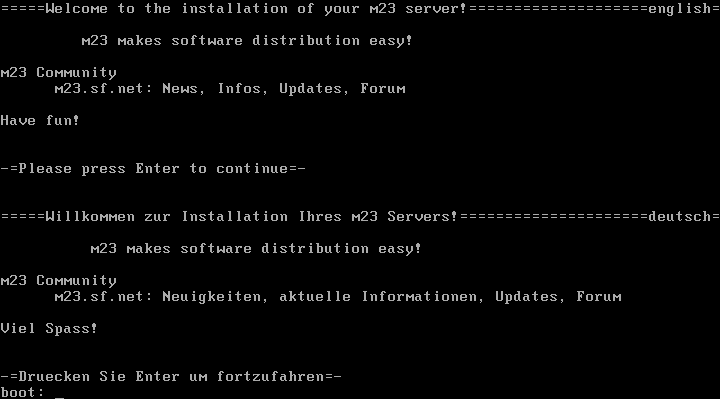
\includegraphics[scale=0.45]{/mdk/doc/manual/screenshots/serverinstall/de/inst1.png}\\
Dies ist der Bootbildschirm der m23-Server-Installations-CD. Nach Dr�cken der Enter-Taste bootet das Linux-Betriebssystem von der CD und startet das Installationsprogramm.



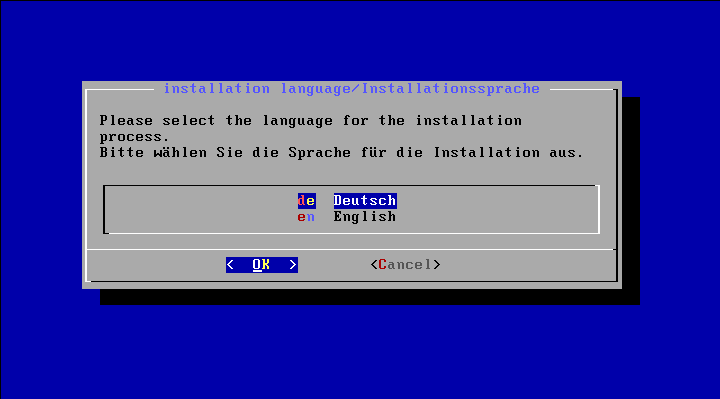
\includegraphics[scale=0.45]{/mdk/doc/manual/screenshots/serverinstall/de/inst2.png}\\
Sie k�nnen w�hlen, ob Sie das Installationsprogramm in deutscher oder englischer Sprache ausf�hren wollen. Wir gehen hier davon aus, da� Sie sich f�r deutsch entscheiden.



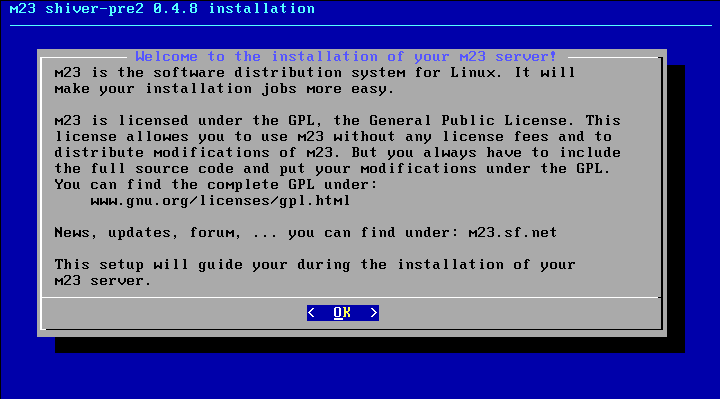
\includegraphics[scale=0.45]{/mdk/doc/manual/screenshots/serverinstall/de/inst3.png}\\
Eine kleine Begr��ung.



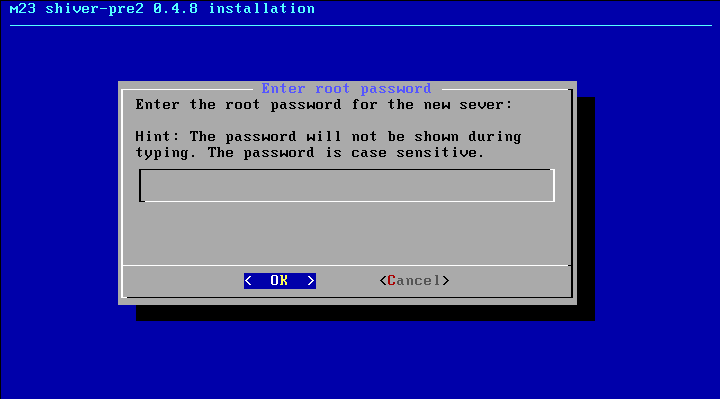
\includegraphics[scale=0.45]{/mdk/doc/manual/screenshots/serverinstall/de/inst4.png}\\
Eingabe des Root-Pa�wortes. Root ist der Systemadministrator mit uneingeschr�nktem Zugriff auf den m23-Server. Sie sollten ein Pa�wort w�hlen, das nicht leicht erraten werden kann und mindestens 10 Zeichen enth�lt. Ebenfalls sollten Sie Sonderzeichen, Ziffern, sowie Gro�- und Kleinschreibung verwenden.\\
Da das Pa�wort nicht angezeigt wird, wird es im darauffolgenden Dialog noch einmal durch erneute Eingabe �berpr�ft.



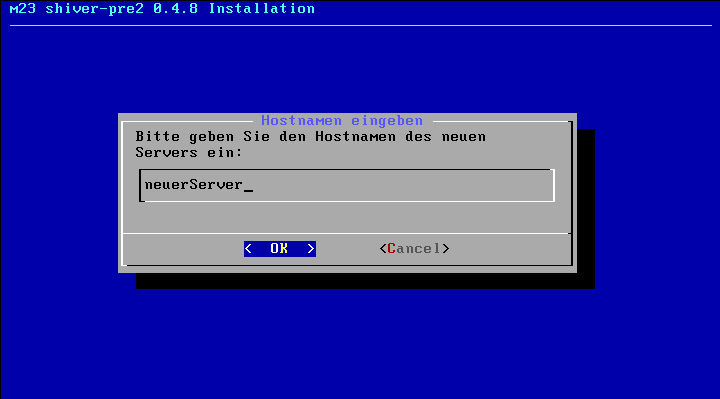
\includegraphics[scale=0.45]{/mdk/doc/manual/screenshots/serverinstall/de/inst5.png}\\
Der Hostname ist der Name f�r den Server. Was f�r eine Erkl�rung ;)



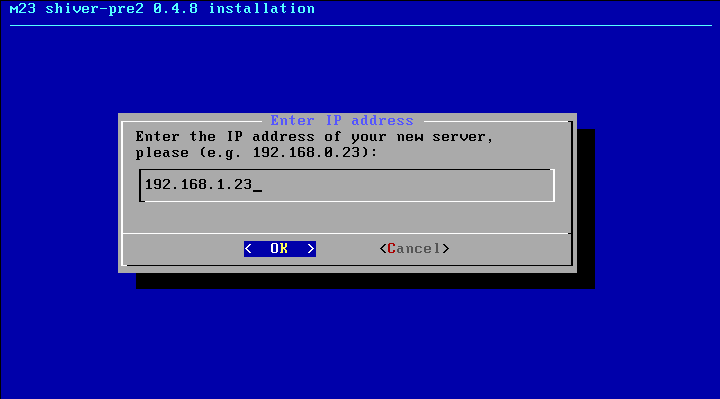
\includegraphics[scale=0.45]{/mdk/doc/manual/screenshots/serverinstall/de/inst6.png}
\\
Die IP-Adresse, unter der auf den Server zugegriffen werden soll. Diese Adresse sollte so gew�hlt werden, da� die Clients von dem Server ohne Router erreicht werden k�nnen.



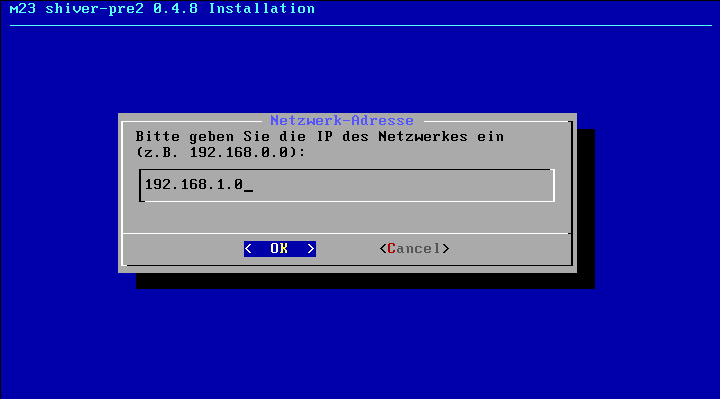
\includegraphics[scale=0.45]{/mdk/doc/manual/screenshots/serverinstall/de/inst7.png}\\
Die Netzwerk-Adresse ist die IP-Adresse, unter der das Netzwerk erreichbar ist.



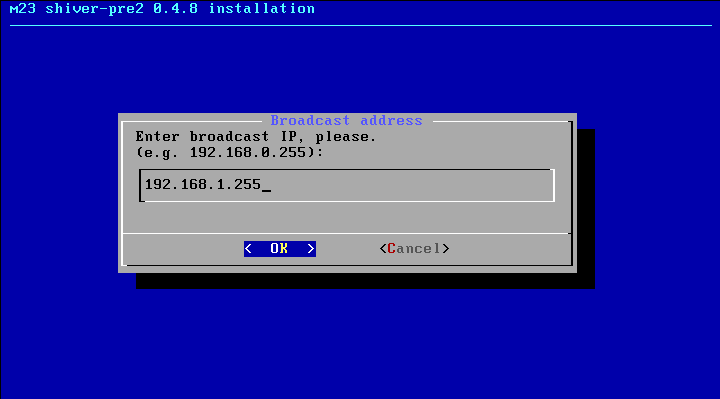
\includegraphics[scale=0.45]{/mdk/doc/manual/screenshots/serverinstall/de/inst8.png}
\\



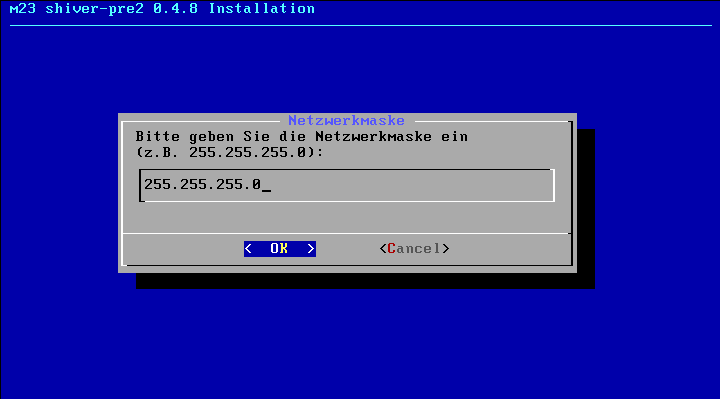
\includegraphics[scale=0.45]{/mdk/doc/manual/screenshots/serverinstall/de/inst9.png}
\\
Die Netzwerkmaske gibt an, welcher Teil der IP zu den einzelnen Rechnern geh�rt und welcher das Netzwerk maskiert.



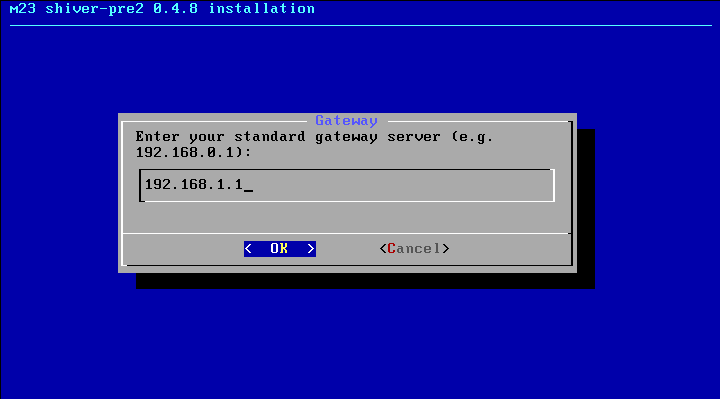
\includegraphics[scale=0.45]{/mdk/doc/manual/screenshots/serverinstall/de/inst10.png}
\\
Die Gateway-IP gibt die IP an, �ber die Anfragen an IPs geleitet werden, die nicht innerhalb des Netzwerkes des Servers liegen. Dies wird vor allem f�r den Zugriff auf das Internet ben�tigt.



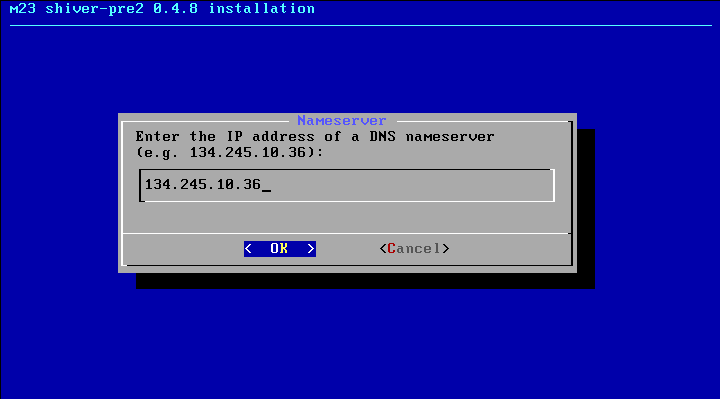
\includegraphics[scale=0.45]{/mdk/doc/manual/screenshots/serverinstall/de/inst11.png}
\\
F�r die Aufl�sung von URL-Namen in IP-Adressen wird ein DNS-Server ben�tigt, der die Umwandlung vornimmt. Aus ftp.debian.org wird z.B. 128.101.80.131. Falls Sie keinen DNS-Server kennen, k�nnen Sie die IP 134.245.10.36 benutzen. Dies ist der DNS-Server der Universit�t Kiel.



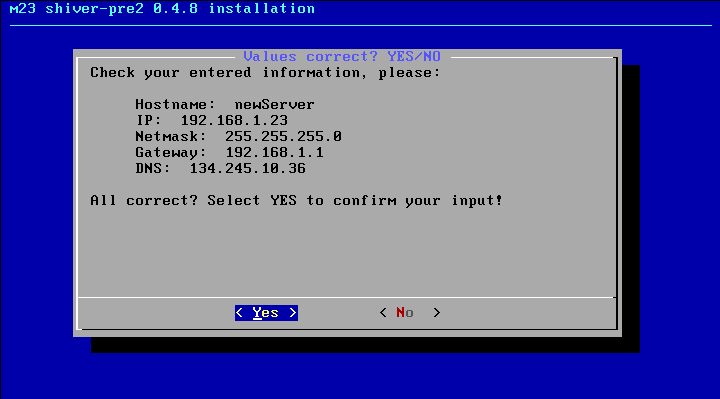
\includegraphics[scale=0.45]{/mdk/doc/manual/screenshots/serverinstall/de/inst12.png}
\\
An dieser Stelle haben Sie noch einmal die M�glichkeit, zu �berpr�fen, ob Ihre Angaben alle korrekt sind. Falls Sie die Installation fortsetzen m�chten, dann w�hlen Sie "Yes", ansonsten k�nnen Sie nach der Auswahl von "No" die korrigierten Angaben eingeben.



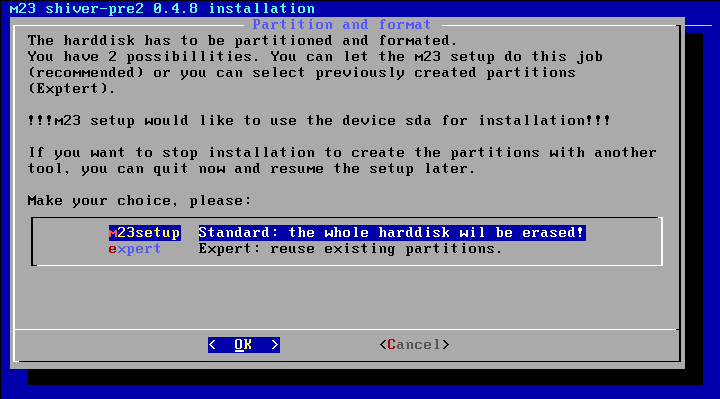
\includegraphics[scale=0.45]{/mdk/doc/manual/screenshots/serverinstall/de/inst13.png}
\\
Hier k�nnen Sie ausw�hlen, ob Sie die komplette Festplatte des Servers f�r m23 verwenden wollen. Dann werden 2 Partitionen eingerichtet, eine f�r das Debian-Linux-Betriebssystem und eine als Swapbereich. Sollten mehrere Festplatten vorhanden sein, so wird die erste benutzt. Sie k�nnen allerdings auch zuvor angelegte Partitionen verwenden, falls Sie eine spezielle Partitionierung w�nschen.\\\\
\underline{Hinweise zur Partitionierung}
Bitte beachten Sie, da� w�hrend der Installation entweder der Server komplett gel�scht wird, oder Sie vorher mit einem Programm wie Parted, fdisk, cfdisk etc. zwei Partitionen der ersten Festplatte (hda bzw. sda) wie folgt erstellen m�ssen:
\begin{itemize}
\item eine Partition f�r m23 mit einer Gr��e von mindestens 4 GB
\item eine Partition zum Swappen f�r Linux (Empfohlen ist hier die doppelte Gr��e des Arbeitsspeichers)
\end{itemize}
Schreiben Sie sich bitte die Adressen der Partitionen auf, d.h. die erste Partition der ersten Festplatte hei�t z.B. hda1, die zweite Partition hda2. Wenn Sie eine Erweiterte- bzw. Extended-Partition benutzen, dann hei�t die erste Partition innerhalb der Erweiterten-Partition hda5 und die zweite hda6 usw. Sie werden w�hrend der Installation nach diesen Adressen gefragt, sofern Sie die Experten-Einstellung zum Partitionieren gew�hlt haben.
Wir empfehlen f�r die meisten Benutzer allerdings, die Daten vorher zu sichern und m23 den kompletten Server partitionieren und formatieren zu lassen.



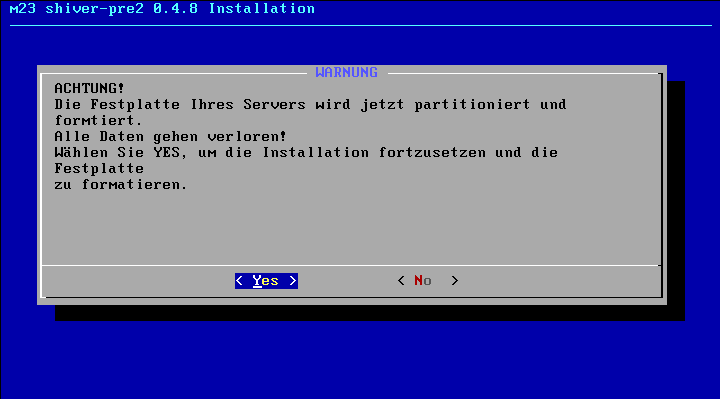
\includegraphics[scale=0.45]{/mdk/doc/manual/screenshots/serverinstall/de/inst14.png}
\\
Die letzte Warnung, bevor es losgeht ;)



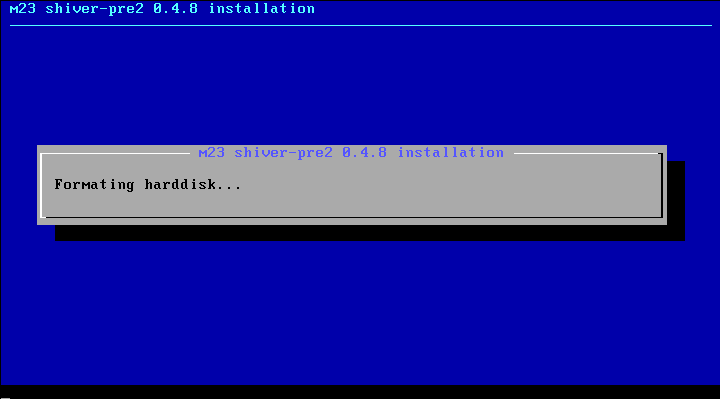
\includegraphics[scale=0.45]{/mdk/doc/manual/screenshots/serverinstall/de/inst15.png}
\\



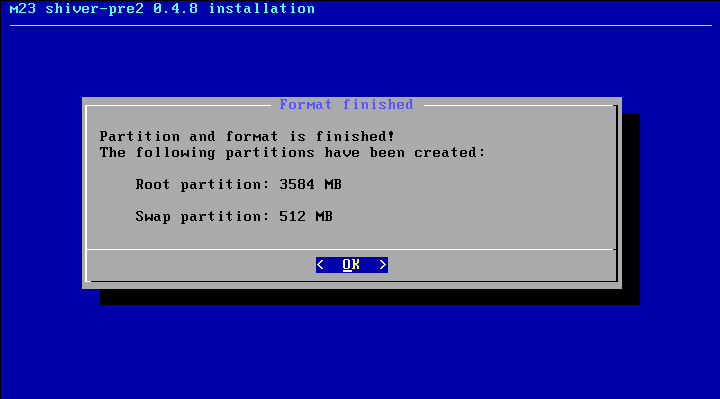
\includegraphics[scale=0.45]{/mdk/doc/manual/screenshots/serverinstall/de/inst16.png}
\\



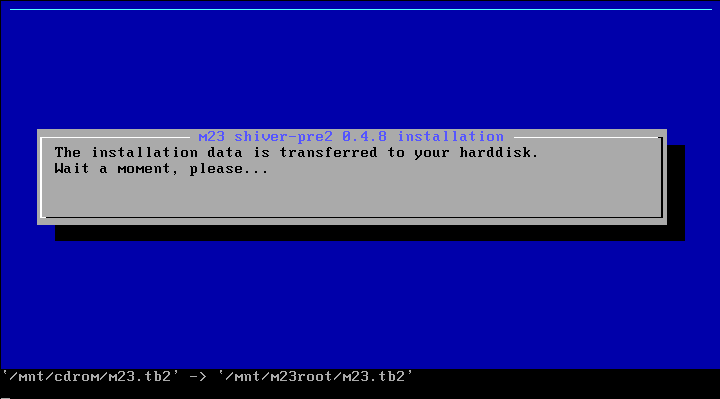
\includegraphics[scale=0.45]{/mdk/doc/manual/screenshots/serverinstall/de/inst17.png}
\\


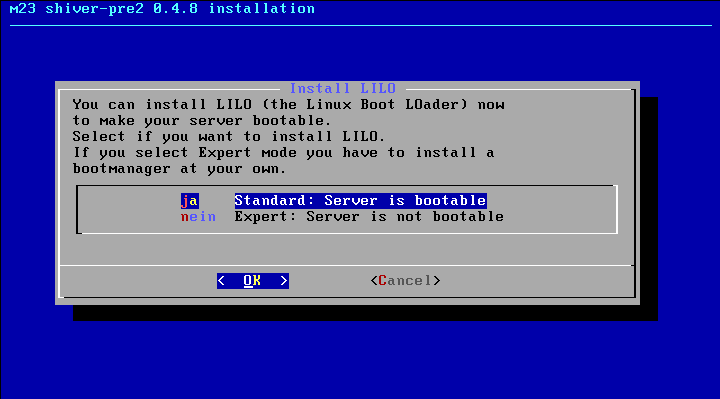
\includegraphics[scale=0.45]{/mdk/doc/manual/screenshots/serverinstall/de/inst18.png}
\\
Hier k�nnen Sie entscheiden, ob Sie den Bootmanager LILO (LInux LOader) installieren wollen. Dieser wird im MBR (MasterBootRecord) der ersten Festplatte installiert. Sollten Sie sich dagegen entscheiden, so m�ssen Sie selbst einen Bootmanager installieren. Ansonsten ist der m23-Server nicht bootf�hig.


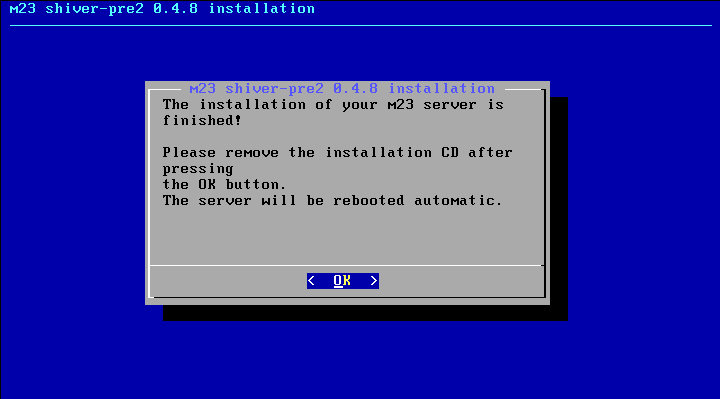
\includegraphics[scale=0.45]{/mdk/doc/manual/screenshots/serverinstall/de/inst19.png}
\\
Die Installation ist abgeschlossen ;)
\section{Abschlu� der Installation}
\underline{Hinweise}: Sie brauchen im normalen Betrieb f�r Ihren m23-Server keinen Monitor, es sei denn Sie m�chten ihn zus�tzlich auch zum Arbeiten benutzen. Da der m23-Server auf ein Debian GNU/Linux-System aufgesetzt ist, k�nnen Sie sich ganz normal mit root und Ihrem bei der Installation eingegebenen Passwort einloggen und sich zus�tzliche Software wie unter Debian �blich installieren. Hierzu verweisen wir auf \underline{www.debian.org}.\\
Nun k�nnen Sie Ihren ersten Client aufsetzen!

\chapter{Erste Schritte mit dem m23-Server}
\section{Verbindung zum m23-Server aufnehmen}
Nachdem Sie Ihren Server erfolgreich installiert und neu gestartet haben, gelangen Sie �ber einen beliebigen Webbrowser auf einem am Netzwerk angeschlossenen PC auf die m23-Administrationsoberfl�che. Geben Sie dazu in Ihrem Webbrowser folgende Ziel-URL ein:\\\\
\underline{http://ServerIP}\\\\

Als ServerIP nehmen Sie bitte die IP Ihres m23-Servers (z.B.: 192.168.1.23). Beim ersten Einloggen haben Sie noch kein eigenes m23-Administrator-Konto, deshalb geben Sie bitte das LOGIN und PASSWORT ein, welches auf der Hintergrundfl�che steht. Sobald Sie eingeloggt sind, sollten Sie sich ein eigenes m23-Administrator-Konto einrichten und das god-Konto l�schen.

\section{Vorgehen beim Hinzuf�gen eines Clients}
Hier wird das allgemeine Vorgehen beim Hinzuf�gen eines neuen Clients beschrieben. F�r die genaue Vorgehensweise sei auf die jeweiligen Kapitel verwiesen.

\begin{itemize}
\item Schlie�en Sie den Client an das Netzwerk an, so da� Client und Server aufeinander zugreifen k�nnen.
\item Erstellen Sie ggf. eine Bootdiskette f�r den Client und legen Sie diese ein. Eine Bootdiskette ben�tigen Sie nur, falls Ihr Client nicht �ber eine Netzwerkkarte mit PXE verf�gt.
\item Starten Sie den Client und notieren Sie sich die MAC-Adresse (z.B. 00:45:23:3A:96:F3).
\item Geben Sie die MAC-Adresse zusammen mit den anderen ben�tigten Daten ein (wie im Kapitel "Clients verwalten" beschrieben) und legen Sie den Client an.
\item Sollte der Client nicht automatisch booten, dann Rebooten Sie ihn und lassen die evtl. erstellte Bootdiskette im Laufwerk.
\item Nun bootet der Client und sendet Hardware- und Partitionierungs-Informationen an dem m23-Server.
\item Im Webinterface k�nnen Sie diese Daten begutachten. Fahren Sie mit dem Kapitel "Clients partitionieren und formatieren" und anschlie�end mit "Installation des Betriebssystems" fort.
\item Zur Installation zus�tzlicher Software schauen Sie in das Kapitel "Pakete installieren/deinstallieren".
\end{itemize}

\chapter{Serveur}
\input{../htaccess.hlp.tex}
\input{../serverupdate.hlp.tex}
\input{../daemonsAndPrograms.hlp.tex}
\input{../ldapSettings.hlp.tex}
\input{../manageGPGKeysDialog.hlp.tex}
\input{../manageImageFiles.hlp.tex}
	\input{../serverBackup.hlp.tex}
	\input{../serverBackupList.hlp.tex}
	\input{../serverRestore.hlp.tex}
\input{../ipManagement.hlp.tex}

\chapter{Service de t�l�administration de m23}
\input{../RASInstalled.hlp.tex}
\input{../RASNotInstalled.hlp.tex}

\chapter{Administrer des clients}
\section{Vue d'ensemble des postes client}Sur cette page, vous voyez une liste de vos postes client.\\
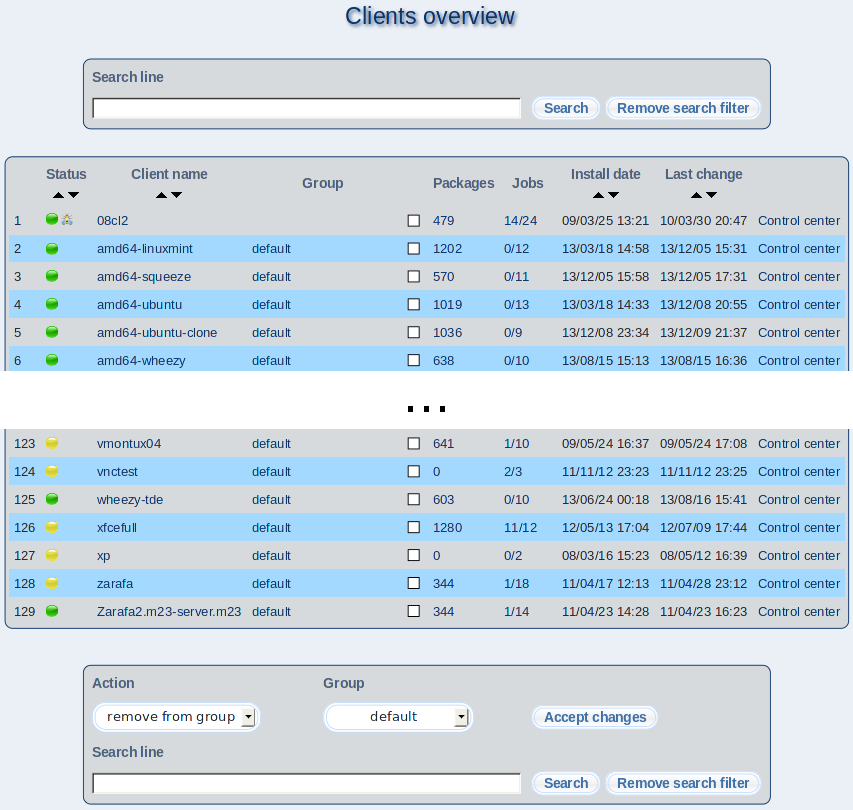
\includegraphics[scale=0.4]{/mdk/doc/manual/screenshots/fr/clients_overview.png} \\
Quand vous cliquez sur le nom d'un client, vous recevrez des informations d�taill�es sur le client s�lectionn� et vous auriez acc�s au centre de contr�le.\\
\subsection{Signification des couleurs symboliques}
Le couleur du symbol d'�tat indique l'�tat de l'installation du poste client.\\
\begin{itemize}
\item \textbf{rouge}: Le poste client a �t� ajout� et la d�tection du mat�riel automatique n'est pas encore termin�e.\\
\item \textbf{jaune}: Vous pouvez formater et partitionner le poste client, le syst�me de base sera assign� automatiquement.\\
\item \textbf{vert}: Le syst�me de base du poste client est �tabli et vous pouvez installer du logiciel suppl�mentaire.\\
\item \textbf{bleu}: Le poste client est en train d'installer du logiciel suppl�mentaire.\\
\item \textbf{orange}: Le poste client est dans un \textbf{�tat critique}. Cela veut dire qu'il y a eu une erreur pendant l'installation qui doit �tre �cart�e par l'administrateur. Au centre de contr�le, il y a des possibilit�s diff�rentes d'�carter l'�tat critique.\\
\item \textbf{blanc}: Poste client mod�le pour l'installation de masse dont les configurations seront transmis aux autres postes client.\\
\item \textbf{Mouche (bogue)}: Indique que le poste client se trouve en �tat de d�bogage.\\
\end{itemize}
\subsection{Travaux}
Dans cette colonne, vous trouvez le nombre des t�ches pas encore acomplies devant et le nombre de toutes les t�ches apr�s la barre oblique.\\
\subsection{Travailler plusieurs postes clients}
Vous pouvez choisir plusieurs postes client en mettant un crochet dans la colonne avec les postes clients souhait�s.\\
Puis, vous pouvez exercer des actions diff�rentes avec les postes client choisis:\\
\begin{itemize}
	\item \textbf{Effacer d'un groupe}: S�lectionnez le groupe duquel vous voulez effacer les postes client. Si un poste client n'appartient pas � ce groupe, aucune action sera excerc� avec lui.\\
	\item \textbf{Ajouter � un groupe}: S�lectionnez le groupe auquel vous voulez ajouter les postes client. Si un poste client appartient d�j� � ce groupe, rien ne sera chang� � sa d�pendance.\\
	\item \textbf{Effacer}: Efface les postes client s�lectionn�s\\
\end{itemize}
\subsection{Notez}
Pour voir l'�tat actuel de vos postes client, utilisez la fonction de rechargement de votre navigateur web (par exemple en appuyant sur la touche F5)\\
\subsection{Astuces}
En cliquant sur le symbole d'�tat d'un poste client, vous pouvez changer l'�tat actuel du poste client. Quand m�me, vous devriez seulement changer l'�tat d'un poste client si vous savez exactement ce que vous faites.\\
Le mode de d�bogage peut �tre (d�s)activ� par un clic sur le symbole avec la mouche.\\


	%control center
	\input{../clientdetails.hlp.tex}
		\section{Hardware information}Here you can see information about the hardware of the selected client.\\
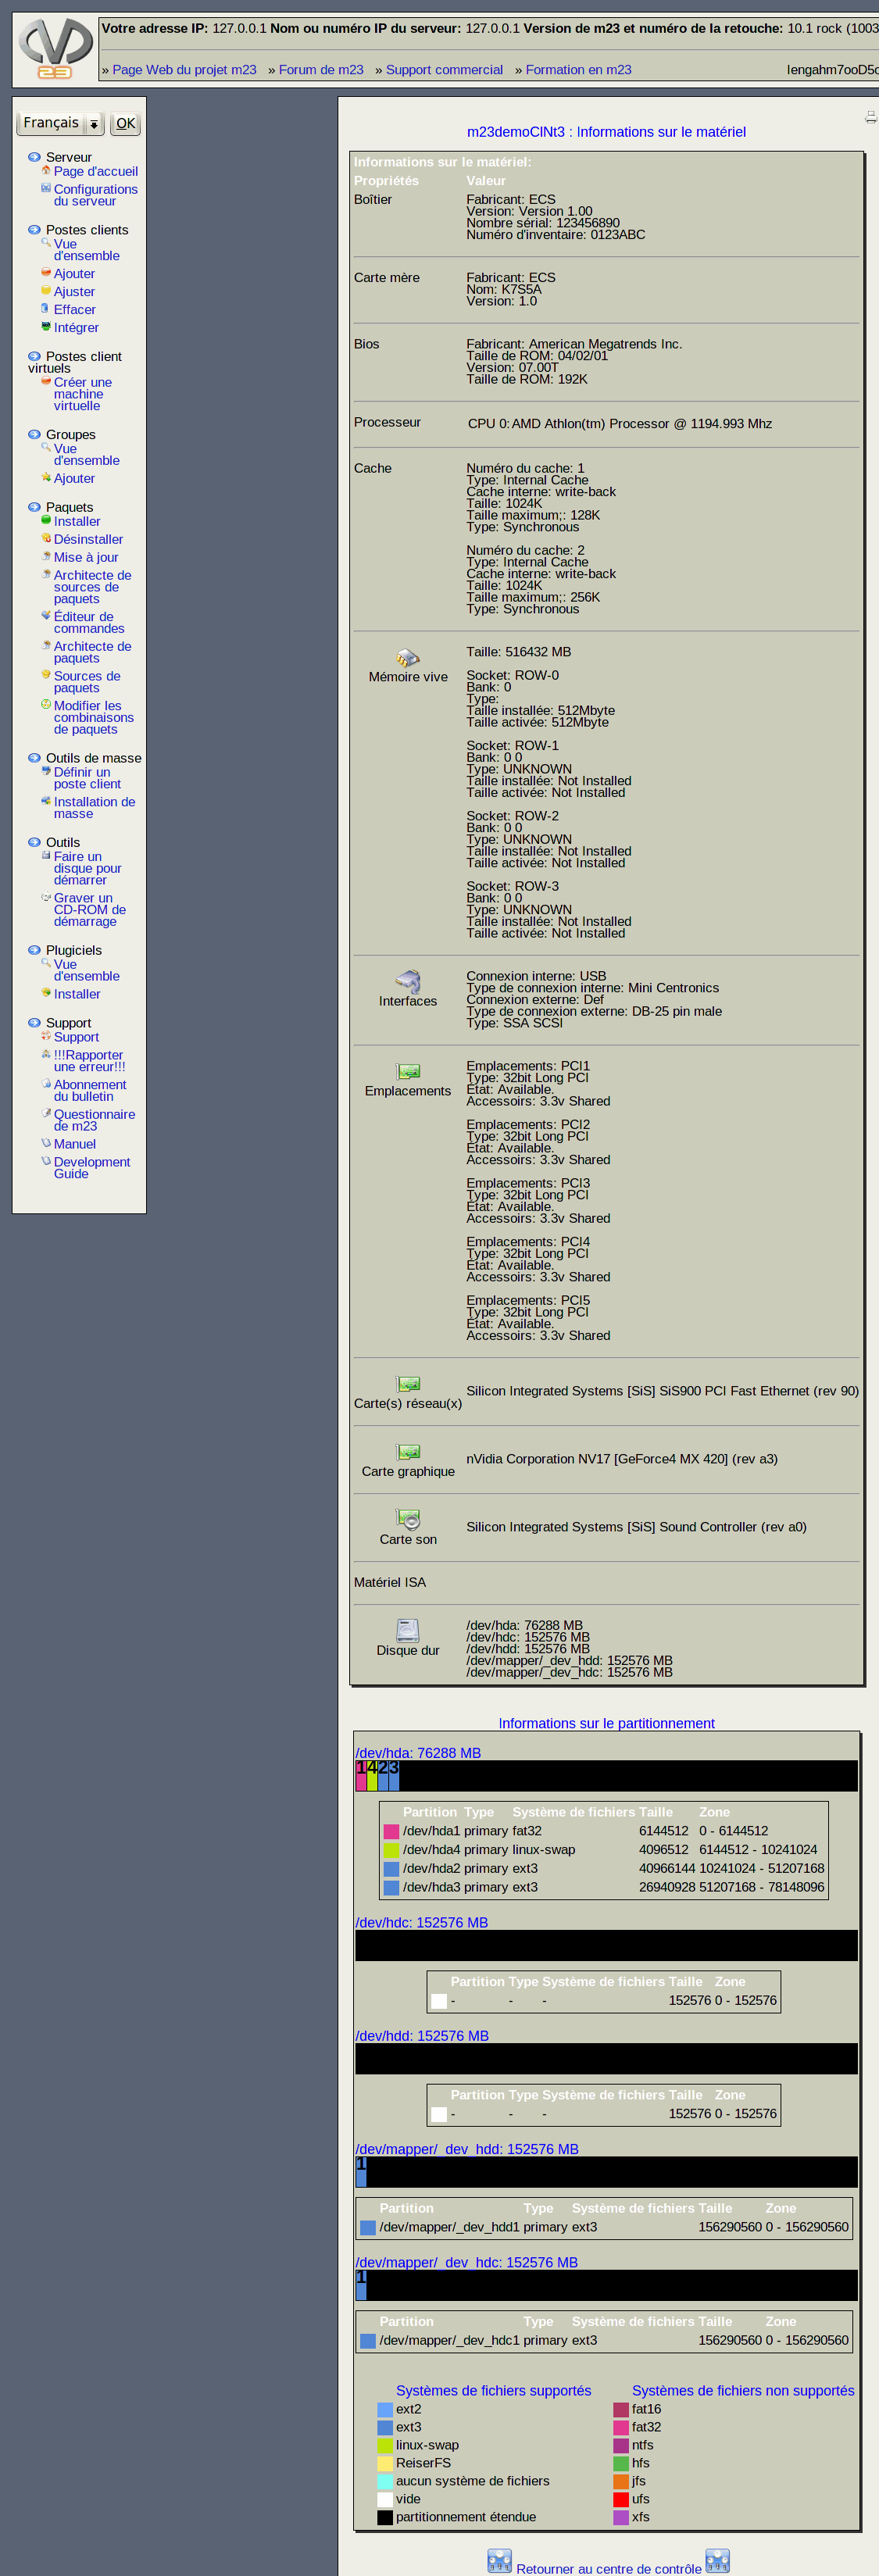
\includegraphics[scale=0.25]{/mdk/doc/manual/screenshots/en/clientinfo_hardware.png} \\

		\section{Paquets}Ici, vous pouvez chercher des paquets qui sont install\'es sur le client. Quand vous voulez voir tous les paquets, n'entrez rien et cliquez sur \textit{$\ll$Rechercher$\gg$}.\\
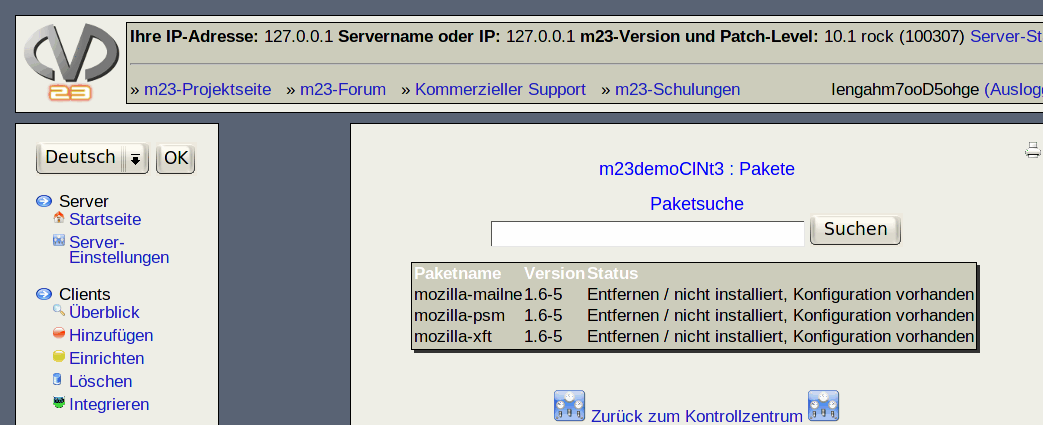
\includegraphics[scale=0.4]{/mdk/doc/manual/screenshots/fr/clients_packages.png} \\

		\section{Protocole du poste client}Dans ce protocole, vous pouvez voir des informations sur les installations et d\'esinstallations et des autres actions ex\'ecut\'ees sur votre poste client.\\
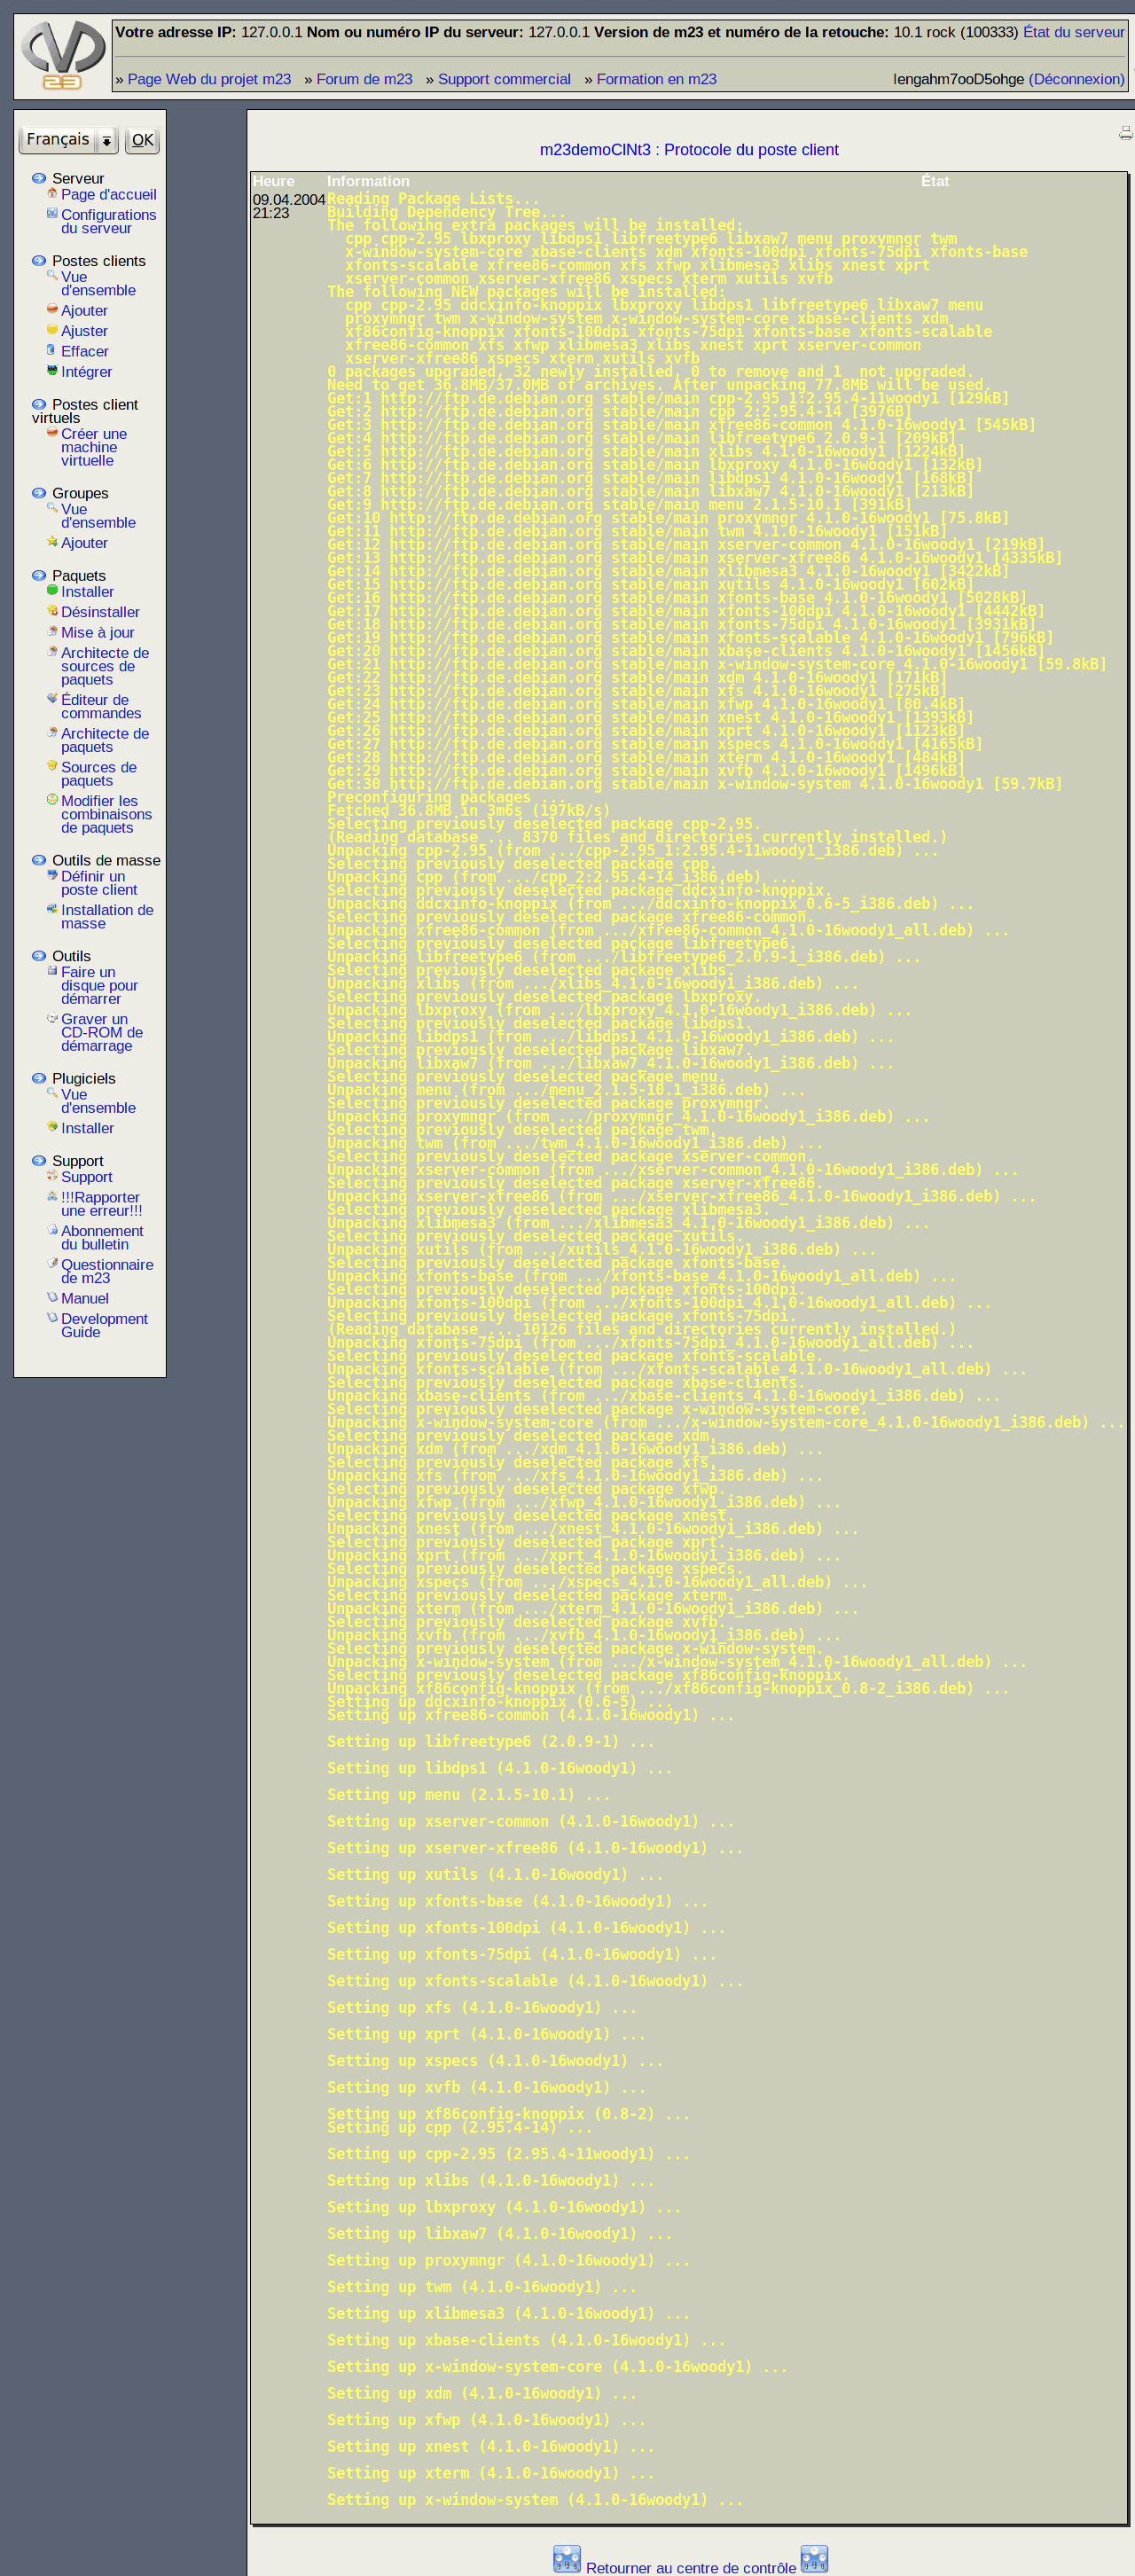
\includegraphics[scale=0.4]{/mdk/doc/manual/screenshots/fr/clientinfo_clientLog.png} \\

		\section{Add to group}Select the groups by checking you want the client to be added to. Click on \textit{"Add"} afterwards.\\
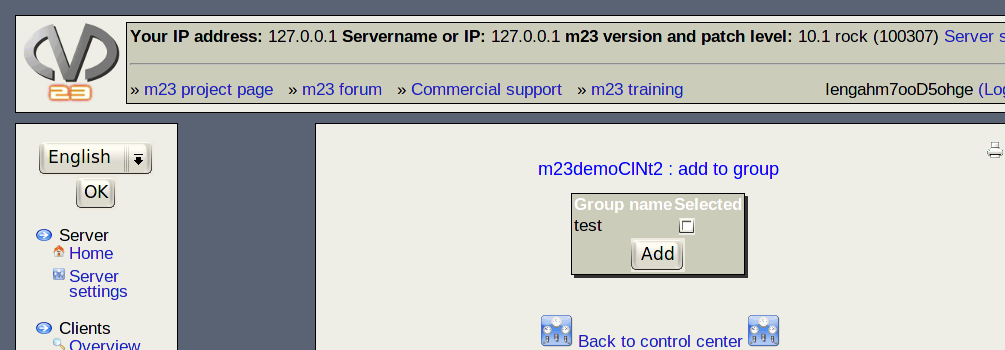
\includegraphics[scale=0.4]{/mdk/doc/manual/screenshots/en/clientinfo_addToGroup.png} \\

		\section{Aus Gruppe l�schen}W�hlen Sie die Gruppen durch Ankreuzen aus, aus denen der Client gel�scht werden soll und klicken anschlie�end auf \textit{"L�schen"}.\\
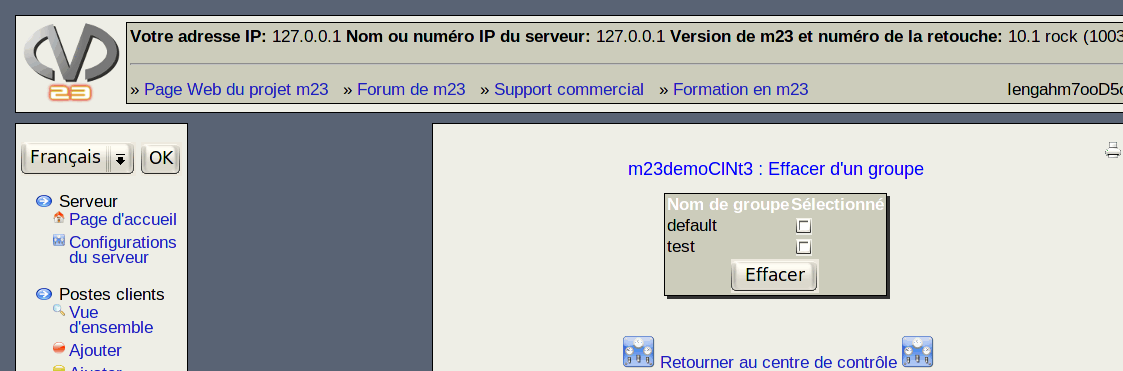
\includegraphics[scale=0.4]{/mdk/doc/manual/screenshots/de/clientinfo_delFromGroup.png} \\

		\section{Recover client}If you want to recover a client, the client will be installed as before. This includes repartitioning and reformatting. All the software which was installed with m23 will be reinstalled. Changes made to the client by hand can't be recovered.\\
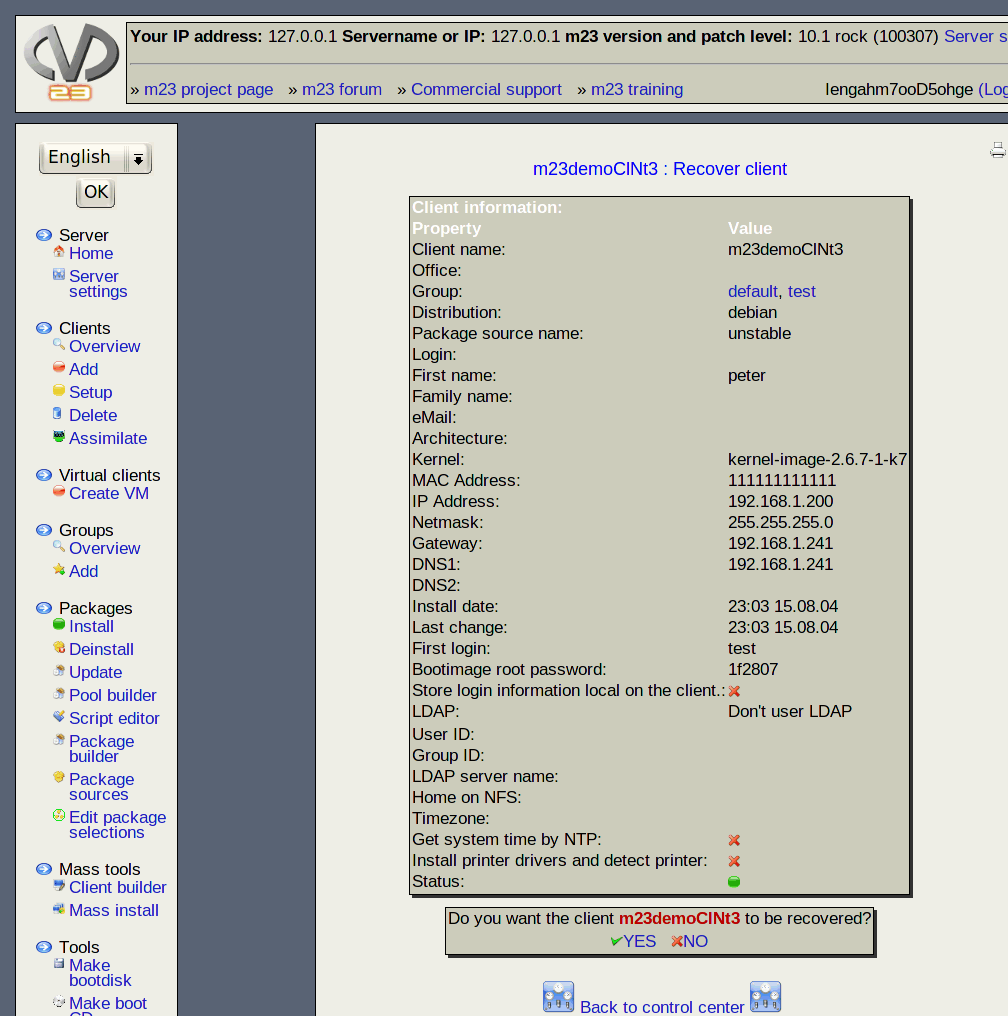
\includegraphics[scale=0.4]{/mdk/doc/manual/screenshots/en/clients_recover.png} \\
\subsection{Hint}
Personal files of the client user can't be recovered.\\

		\section{Start rescue system}If you want to start a client for repairing or diagnostic purpose, you can boot the rescue system over the network. After the network boot the client starts a console that allows you to do your work. To start the rescue system click on \textit{"Rescue system"} after the client name.\\
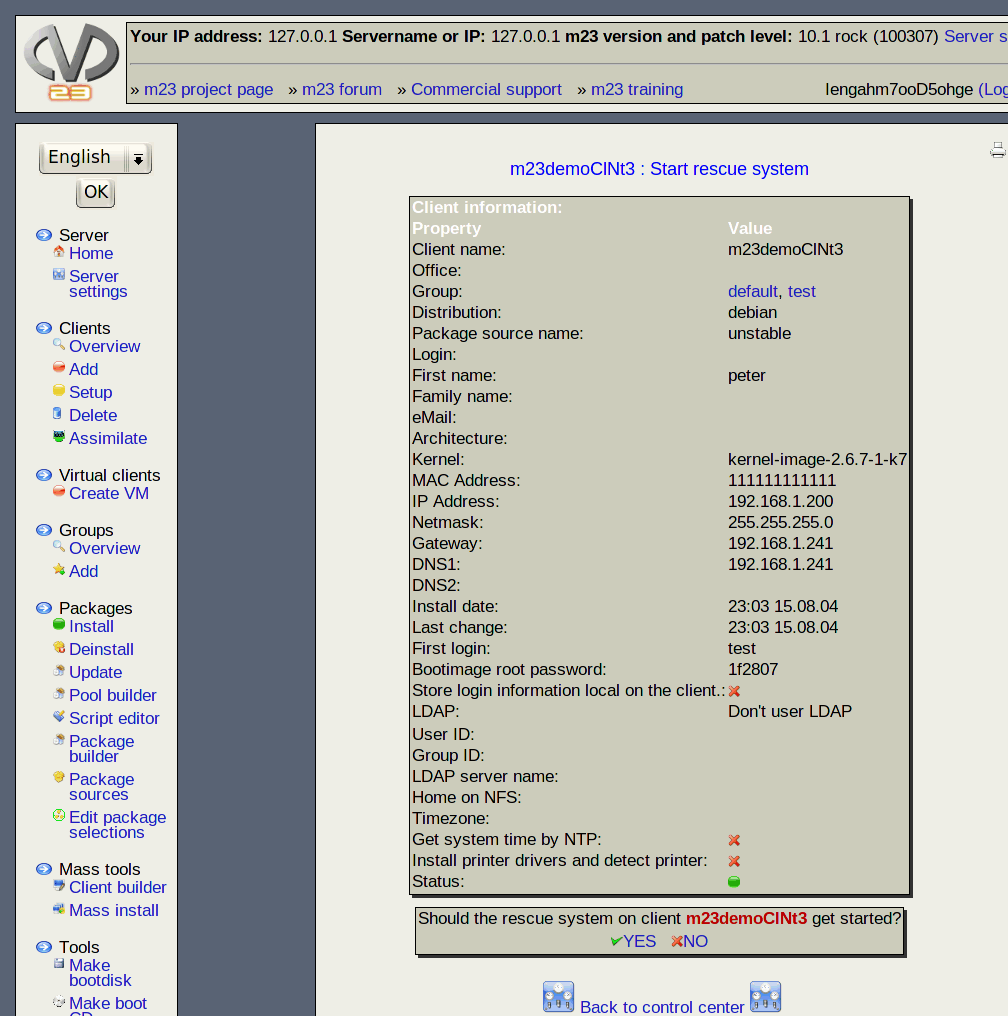
\includegraphics[scale=0.4]{/mdk/doc/manual/screenshots/en/rescue_client.png} \\
\subsection{Hint}:\\
The rescue system will be started every time you boot the client until you delete the "m23Rescue" job from the job list. You can find the list  on the page \textit{"Clients overview"} if you click on the number in the "Jobs" line.\\

		\section{Client-Status �ndern}Hier k�nnen Sie den Status des Clients �ndern. Dies kann z.B. zu Debug-Zwecken oder aus anderen Gr�nden sinnvoll sein.\\
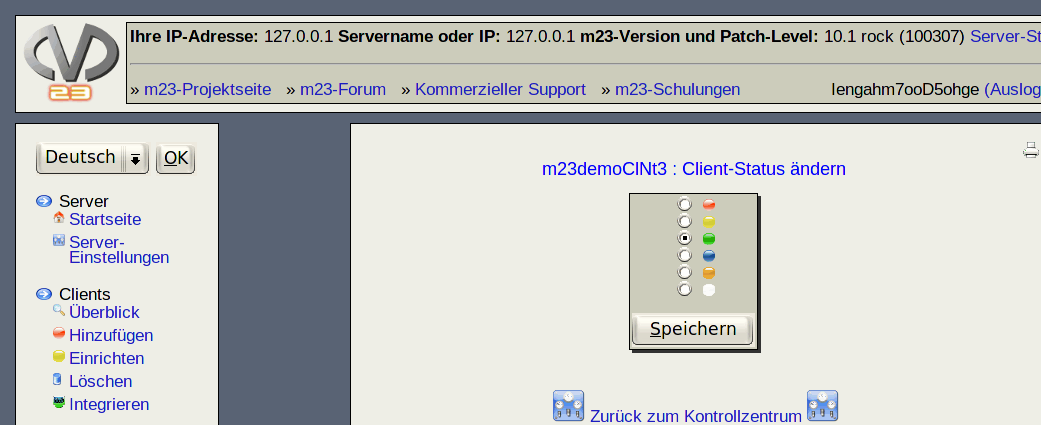
\includegraphics[scale=0.4]{/mdk/doc/manual/screenshots/de/client_status.png} \\
\subsection{Hinweis}
�ndern Sie den Status nur, wenn Sie wissen, was Sie tun.\\

		\section{Changer l'\'etat du d\'ebogage}Des postest client avec le mode de d\'ebogage activ\'e n'indiquent pas d'informations sur l'\'etat de l'utilisateur sur le moniteur, mais les donn\'ees de sortie du script ex\'ecut\'e et des programmes utilis\'es.\\
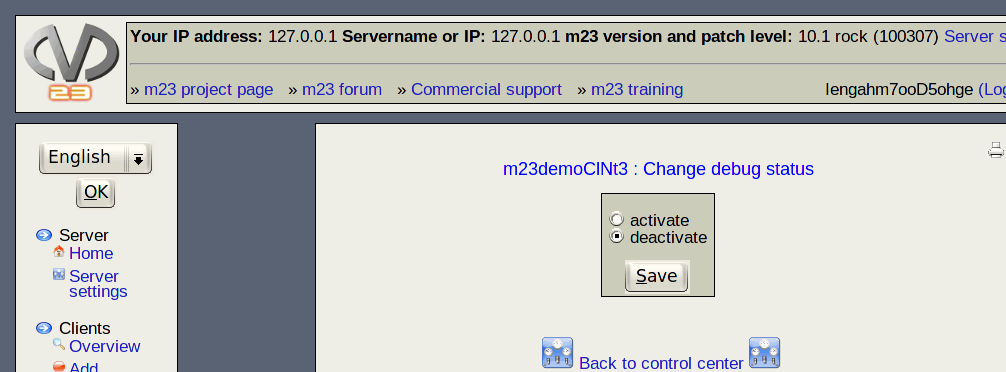
\includegraphics[scale=0.4]{/mdk/doc/manual/screenshots/fr/client_debug.png} \\
Comme �a, vous pouvez mieux voir s'il y a des erreur ex\'ecutant le script.\\

		\section{Client-Direkt-Verbindung}Eine Client-Direkt-Verbindung kann dazu verwendet werden, um manuell in den Installations-Proze� eines Clients einzugreifen, oder die Bildschirmausgabe von einem entfernten Ort aus zu lesen, sowie zu Test- und Debug-Zwecken. Die Verbindung wird per SSH aufgebaut und kann so mit jedem SSH-Client hergestellt werden.\\

\includegraphics[scale=0.4]{/mdk/doc/manual/screenshots/de/client_directConnection.png} \\
\subsection{Pa�wort}
Ist der Client noch in einem fr�hen Installationsstadium, so lautet das Root-Pa�wort: "NETROOTPWD"\\
Sp�ter ist es das Pa�wort, das Sie beim Anlegen des Clients vergeben haben.\\
Sollte Ihr Browser das SSH-Protokoll direkt unterst�tzen, so k�nnen Sie die Verbindung durch Anklicken dieses Links herstellen: ssh://root@CLIENTIP\\
Sonst �ffnen Sie bitte eine Konsole und geben den Befehl: \textbf{ssh -o UserKnownHostsFile=/dev/null -l root CLIENTIP}
Um in die aktuelle Client-Bildschirmausgabe zu lesen oder in die laufende Installation einzugreifen benutzen Sie den Befehl: \textbf{screen -x m23install}

		\section{Modifier un poste client}Par ce dialogue, vous pouvez modifier la configuration d'un poste client. A part des champs de saisie que vous connaissez d\'ej\`a du dialogue d'ajout d'un poste client, il y a trois colonnes o\`u vous pouvez indiquer ce qui se doit passer avec les valeurs y entr\'ees.\\
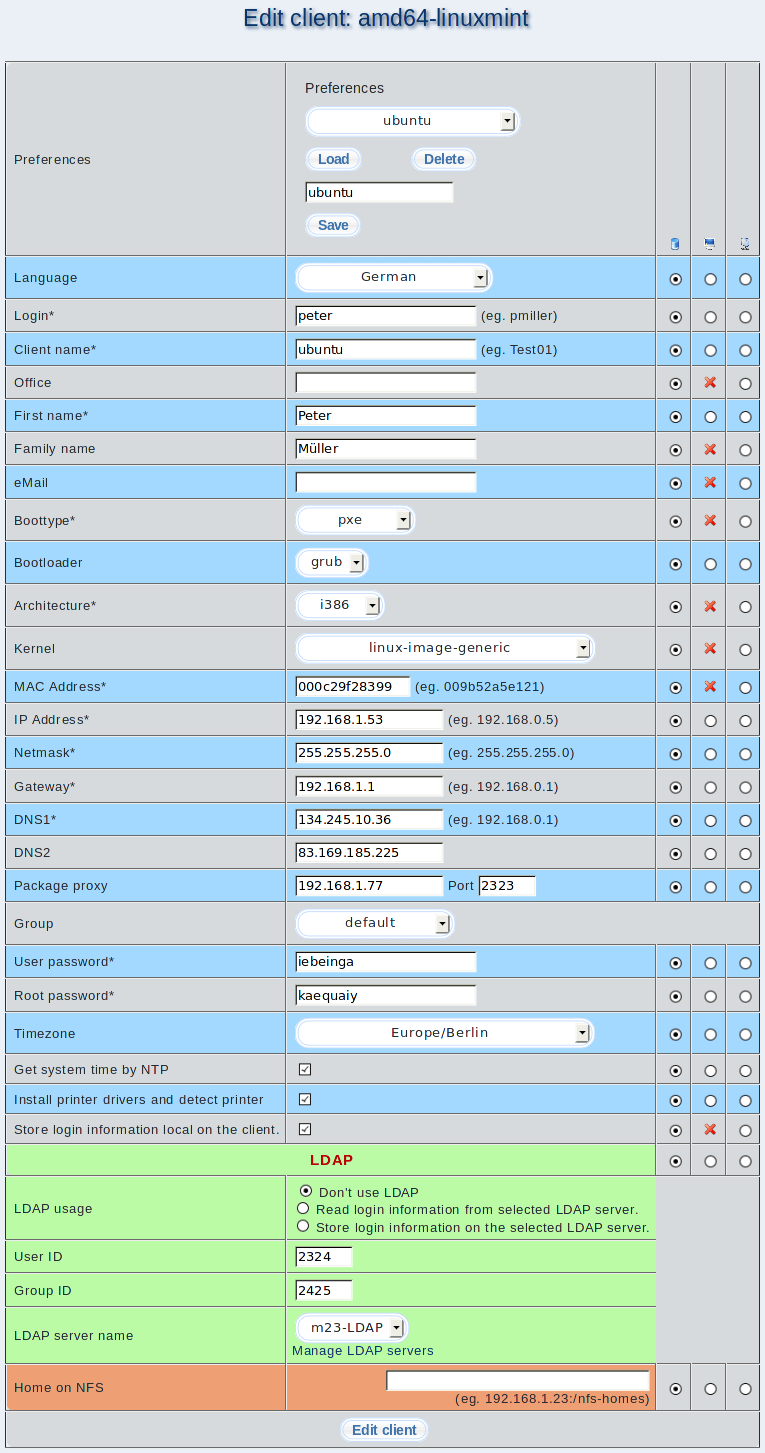
\includegraphics[scale=0.4]{/mdk/doc/manual/screenshots/fr/edit_client.png} \\
\begin{itemize}
\item \textbf{Colonne gauche}: Si vous s\'electionnez cette colonne, la valeur enregistr\'ee sur le poste client et le serveur restera inchang\'ee.\\
\item \textbf{Colonne au milieu}: Les changements doivent \^etre ex\'ecut\'es sur le poste client et apr\`es, les donn\'ees sur le serveur seront actualis\'ees.\\
\item \textbf{Colonne droite}: Seul les valeurs dans la banque de donn\'ees sur le serveur seront chang\'ees. Ceci est utile, par exemple, quand les changements sur le poste client ont d\'ej\`a \'et\'es ex\'ecut\'es \`a la main.\\
\end{itemize}
\subsection{Notez}
Certaines configurations seront enregistr\'ees seulement sur le serveur. Pour cette raison, une modification sur le poste client n'est pas possible. La colonne au milieu ne peut pas \^etre s\'electionn\'ee pour ces configurations.\\

		\section{Auftr�ge �ndern}
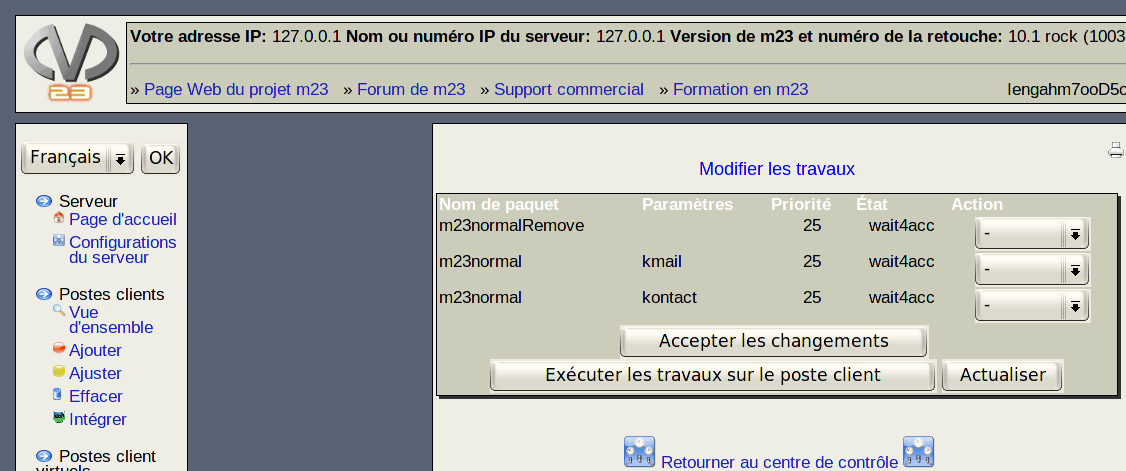
\includegraphics[scale=0.4]{/mdk/doc/manual/screenshots/de/client_changejobs.png} \\
Hier k�nnen Sie bereits abgearbeitete und wartende Auftr�ge des Clients begutachten und ggf. �ndern. Es stehen Ihnen folgende �nderungsm�glichkeiten zur Verf�gung:\\
\begin{itemize}
	\item W�hlen Sie bei \textit{"Aktion"} \textbf{L�schen} aus, um den Auftrag endg�ltig zu verwerfen.\\
	\item \textbf{Wiederholen} setzt einen bereits abgearbeiteten Auftrag wieder auf die Liste der auszuf�hrenden Auftr�ge.\\
	\item \textbf{Fertig} markiert einen Auftrag als abgeschlossen. Dieser wird deshalb nicht mehr ausgef�hrt.\\
\end{itemize}
Klicken Sie anschlie�end auf \textit{"�nderungen �bernehmen"}, um die �nderungen durchzuf�hren. M�chten Sie zus�tzlich, da� die von Ihnen auf \textbf{Wiederholen} gesetzte Auftr�ge sofort ausgef�hrt werden, so klicken Sie auf \textit{"Auftr�ge auf dem Client ausf�hren"}.\\

		\section{Create image}
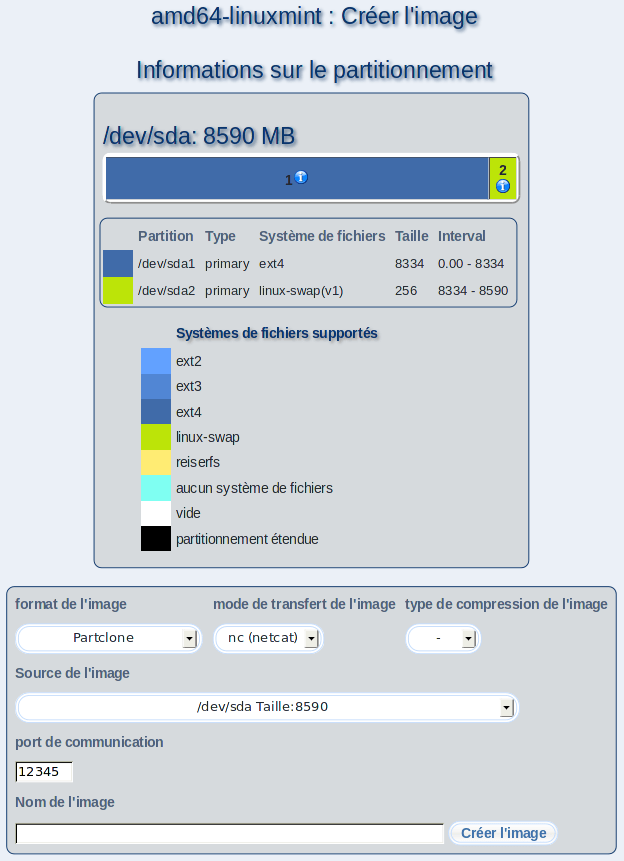
\includegraphics[scale=0.4]{/mdk/doc/manual/screenshots/en/client_createImage.png} \\
You can create images from a partition or a whole drive of your client in this dialog. This image can be used to install clients. Select your preferred Image format, the Image transfer type and the Image compression. You have to make additional designations under \textit{"Image source"} for some image formats e.g. the partition or drive that should be stored in the image.\\
Choose a name for the image and enter it at \textit{"Image name"}. Click on \textit{"Create image"} afterwards.\\
\subsection{Hint for image files}
The files are stored in the directory \textbf{/m23/data+scripts/clientImages} in different types and with distinct compressions. The file names are always created after the following scheme: $\langle$Image name$\rangle$$\langle$Size of the extracted image in bytes$\rangle$$\langle$Image format$\rangle$$\langle$Compression$\rangle$\\
Image format is one of the following values:\\
\begin{itemize}
\item \textbf{dd}: Saves the whole data of a partition or harddisk.\\
\end{itemize}
For the compression the following is valid:\\
\begin{itemize}
\item (no extension): The image file will be stored with no compression.\\
\item \textbf{gz}: The image will be compressed with  gzip.\\
\item \textbf{bz2}: It will be compressed with bzip2 that compresses better mostly.\\
\end{itemize}
\subsection{Hint for the Transfer port}
You have to enter a network port that can be used on client and server side and is not blocked (e.g. firewall) for the Image transfer type. If you want to create images from multiple clients concurrently you have to choose different port numbers.\\

		\section{Backup}
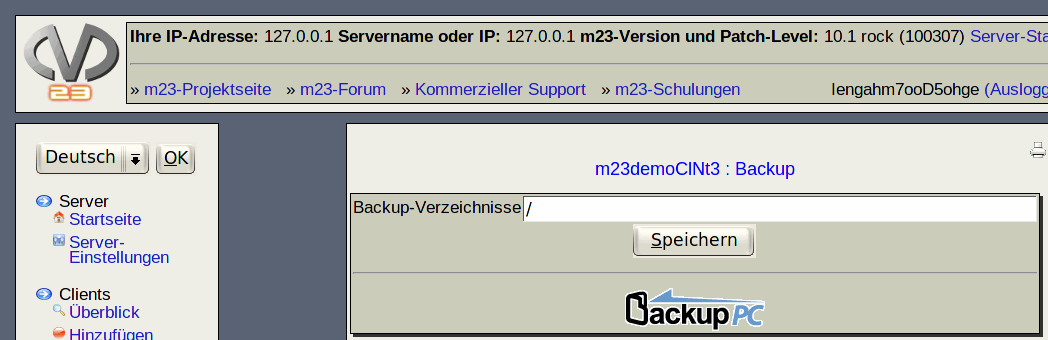
\includegraphics[scale=0.4]{/mdk/doc/manual/screenshots/de/client_backup.png} \\
In diesem Dialog k�nnen Sie alle Verzeichnisse des Clients angeben, von denen ein Backup erstellt werden soll. Geben Sie diese Verzeichnisse dazu durch Kommata getrennt in der Eingabezeile bei \textit{"Backup-Verzeichnisse"} an und klicken Sie anschlie�end auf \textit{"Speichern"}.\\
Das eigentliche Backup �bernimmt das Programm BackupPC, das Sie mit einem Klick auf das Icon starten k�nnen. In der BackupPC-Oberfl�che haben Sie Zugriff auf zus�tzliche Backup-Funktionen.\\


\chapter{Ajuster des clients} %v1.6
\section{Ajouter un poste client}(les champs de saisie marqu\'ees avec * doivent \^etre remplis correctement en tous cas)\\
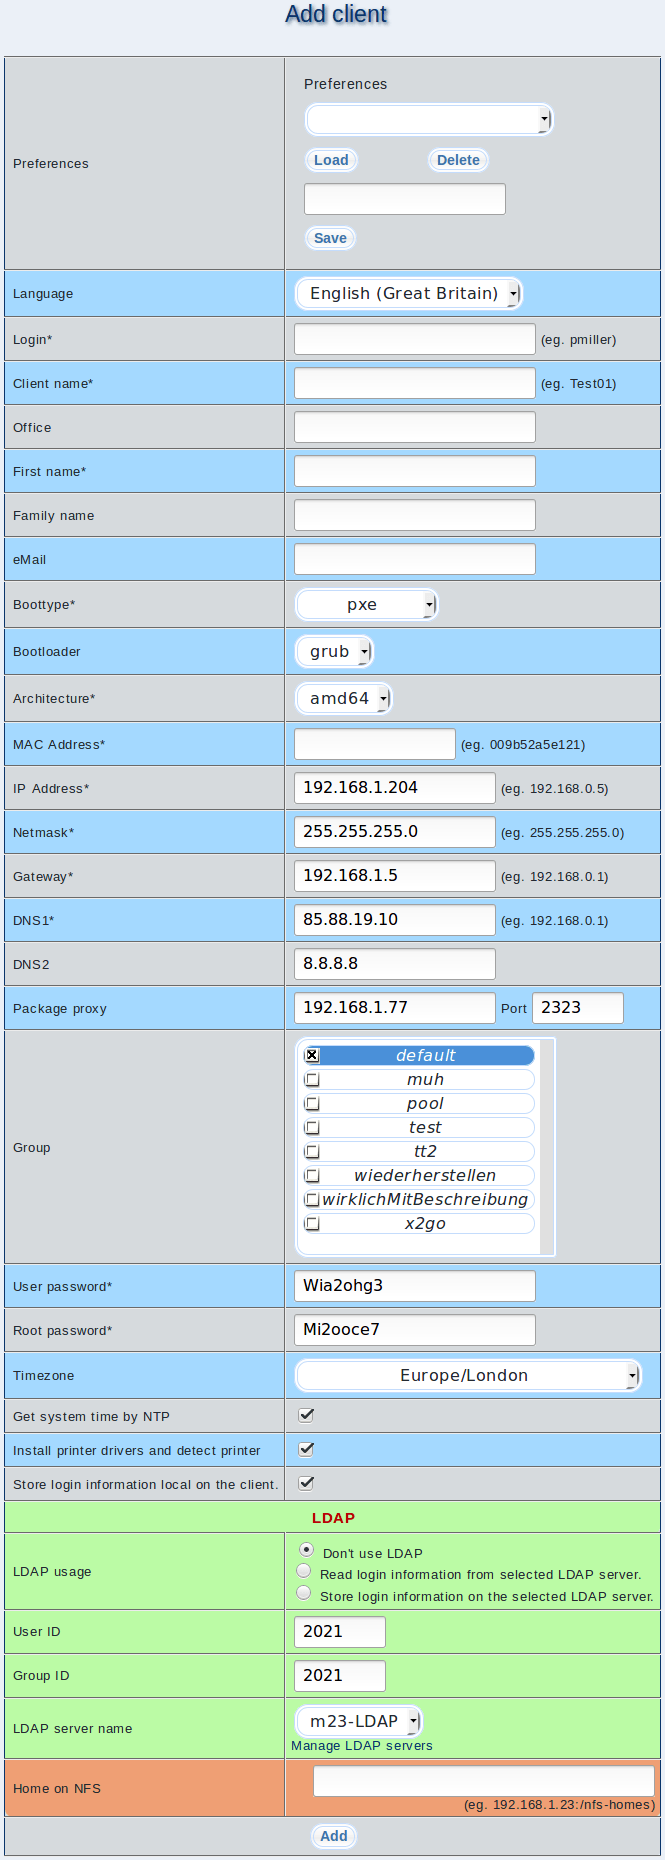
\includegraphics[scale=0.4]{/mdk/doc/manual/screenshots/fr/client_add.png} \\
\begin{itemize}
\item \textbf{Pr�f�rences:} Vous pouvez choisir entre des configurations d\'ej\`a enregistr\'ees et ensuite, vous avez la possibilit\'e de les charger o\`u de les effacer. Si vous voudriez enregistrer la configuration actuelle, entrez un nom pertinent et cliquez sur \textit{$\ll$Enregistrer$\gg$}.\\
\item \textbf{Langue:}Ici vous pouvez choisir la langue pour votre poste client m23. Cette langue sera employ\'ee pour l'ajustement du clavier, du bureau et de la console.\\
\item \textbf{Nom d'entr�e dans le syst�me:} Le nom pour l'entr\'ee dans le syst\`eme du poste client utilis\'e par l'utilisateur.\\
\item \textbf{Nom de poste client:} C'est le nom unique de votre client qui ne devrait pas \^etre employ\'e qu'une fois\\
\item \textbf{Section:} Cette information est volontaire, ici vous pouvez entrer o\`u le client se trouve (par ex. le num\'ero de la chambre etc.)\\
\item \textbf{Langue:} Ici vous pouvez choisir la langue pour votre client. Cette langue sera employ\'ee pour l'installation, pour tous les programmes install\'es, pour le clavier et les options de pays.\\
\item \textbf{Pr�nom:} Pr\'enom de l'utilisateur, correspond au nom d'entr\'ee dans le syst\`eme\\
\item \textbf{Nom de famille:} Nom de famille de l'utilisateur\\
\item \textbf{eMail:} Adresse de courrier \'electronique de l'utilisateur\\
\item \textbf{Type de boot:} Standard de d\'emarrage pour le d\'emarrage des clients vers le r\'eseau. (Notez: Si vous voudriez utiliser m23 avec un serveur DHCP existant, lisez la page suivante: externalDHCP)\\
\item \textbf{Chargeur d'amor�age:} Ici, choisissez quel chargeur d'amor\c{c}age/boot loader vous voudriez utiliser pour l'amor\c{c}age du noyau Linux et des autres syst\`emes d'exploitation eventuellement install\'es. Vous pouvez choisir entre LILO (LInux LOader) et GRUB (GRand Unified Bootloader).\subsection{Information suppl\'ementaire}
La manipulation des param\`etres de d\'emarrage par des personnes non autoris\'ees est emp\^ech\'ee par la protection avec un mot de passe \`a partir de la version m23 0.6.4 . Il est n\'ecessaire d'entrer le mot des passe de d\'emarrage du r\'eseau. Vous pouvez l'extraire dans le centre de contr\^ole sous \textit{$\ll$Connexion directe au poste client$\gg$}.\\
\item \textbf{Architecture du processeur:} Ici, vous pouvez choisir si vous voudriez installer le logiciel pour la version 32 bits ou 64 bits. Regardez aussi le renseignement en bas de la page.\\
\item \textbf{Adresse MAC:} Adresse MAC de la carte r\'eseau du client (par ex. 00:D0:B7:23:86:5C)\\
\item \textbf{Adresse IP:} Adresse IP souhait\'ee du client (par ex. 192.168.1.23)\\
\item \textbf{Masque r�seau:} Masque r\'eseau du r\'eseau (par ex. 255.255.255.0)\\
\item \textbf{Passerelle:} IP de la passerelle pour les connections \`a l'internet ou des autres connections hors du r\'eseau\\
\item \textbf{DNS1:} Adresse IP du serveur DNS pour dissoudre les noms d'internet\\
\item \textbf{DNS2 (facultatif):} Adresse IP du serveur DNS backup\\
\item \textbf{Proxy des paquets:} Le poste client essaie de t\'el\'echarger les paquets de logiciel du num\'ero IP du serveur proxy indiqu\'e. Dans le cas g\'en\'eral, il s'agit du num\'ero IP du serveur m23, mais on peut aussi entrer le num\'ero d'un autre serveur proxy. Si vous laissez ce champs de saisie vide, le client va t\'el\'echarger les paquets de logiciel de l'internet. Entrez \'egalement l'adresse du port du serveur proxy. Au cas du serveur m23, c'est le port 2323. Quand vous ouvrez le dialogue \textit{$\ll$Ajouter un client$\gg$}, le serveur m23 est indiqu\'e comme serveur proxy de standard.\\
\item \textbf{Groupe (facultatif):} Nom du groupe de postes client \`a laquelle appartient le poste client\\
\item \textbf{Mot de passe de l'utilisateur:} C'est le mot de passe de l'utilisateur employ\'e pour la premi\`ere entr\'ee dans le syst\`eme. Ce mot de passe consiste de six chiffres choisis par hasard, mais vous pouvez aussi choisir un autre mot de passe.\\
\item \textbf{Mot de passe de la racine:} C'est le mot de passe qui est employ\'e pour l'acc\`es root au client. Il consiste de huit chiffres choisis par hasard, mais vous pouvez aussi choisir un autre mot de passe.\\
\item \textbf{Fuseau horaire:} Ici, vous pouvez d\'efinir le fuseau horaire, que le poste client doit utiliser.\\
\item \textbf{D�terminer l'heure syst�me par NTP:} S\'electionnez cette option quand vous voudriez que l'heure du poste client doit \^etre accord\'ee par l'internet.\\
\item \textbf{Installer les pilotes de l'imprimante et d�tecter l'imprimante:} Quand vous s\'electionnez cette option, des pilotes d'imprimante seront install\'es et les imprimantes connect\'ees seront d\'etect\'ees.\\
\item \textbf{Enregistrer les donn�es d'ouverture de session local sur le poste client.:}Mettez un crochet ici pour pouvoir utiliser l'entr\'ee dans le syst\`eme locale des postes client.\\
\item \textbf{Ne pas utiliser le LDAP}: Pour pouvoir utiliser l'entr\'ee dans le syst\`eme locale des postes client comme seule option, choisissez \textit{$\ll$Ne pas utiliser le LDAP$\gg$}. \\
\item \textbf{Lire les donn�es d'ouverture de session du serveur LDAP s�lectionn�.}: Si vous voudriez utiliser les donn\'ees d'authentification d'utilisateur enregistr\'ees sur le serveur LDAP, cliquez sur \textit{$\ll$Lire les donn�es d'ouverture de session du serveur LDAP s�lectionn�.$\gg$}.\\
\item \textbf{Enregistrer les donn�es d'ouverture de session sur le serveur LDAP.}: Mais si vous choisissez d'entrer les donn\'ees d'utilisateur indiqu\'ees en haut dans la banque de donn\'ees LDAP du serveur m23 et de les utiliser pour l'entr\'ee dans le syst\`eme sur les postes client, s\'electionnez \textit{$\ll$Enregistrer les donn�es d'ouverture de session sur le serveur LDAP.$\gg$}. Pour pouvoir s\'electionner cette option, il vous faut d'un serveur LDAP avec acc\`es complet, comme les donn\'ees indiqu\'ees en haut seront enregistr\'ees sur le serveur LDAP.\\
\item \textbf{ID de l'utilisateur, ID du groupe}: En plus, vous devez choisir l'\textit{$\ll$ID de l'utilisateur$\gg$} et l'\textit{$\ll$ID du groupe$\gg$} pour l'utilisateur. Ceci est important surtout quand vous voudriez utiliser NFS pour l'enregistrement des r\'epertoires personnels.\\
\item \textbf{Nom du serveur LDAP}: Enfin, vous devez s\'electionner un serveur LDAP de la liste chez \textit{$\ll$Nom du serveur LDAP$\gg$}. Si le serveur LDAP souhait\'e n'y serait pas affich\'e, vous pouvez l'ajouter apr\`es un clic sur \textit{$\ll$Administrer le serveur LDAP$\gg$}.\\
\item \textbf{R�pertoire personnel sur le serveur NFS:} Cette option assure que les donn\'ees d'utilisateur seront enregistr\'ees sur un serveur NFS central, pour qu'elles puissent \^etre acc\'ed\'ees de tout poste client (en combination avec LDAP). Pour activer le NFS, entrez le nom de l'ordinateur ou son adresse IP et le chemin pour l'enregistrement des r\'epertoires personnels, comme par exemple: \\
\begin{verbatim}
192.168.1.42/nfs/home
\end{verbatim}
.\\
\end{itemize}
Veuillez ajouter le client en cliquant sur \textit{$\ll$Ajouter$\gg$}.\\
\subsection{Information suppl\'ementaire:}
Apr\`es \^etre \'etabli, le client parcourt une sequence de d\'etection du mat\'eriel, pendant laquelle des informations, comme par ex. sur la taille du disque dur utilis\'e, sont envoy\'ees au serveur.\\
Apr\`es l'ach\`evement du transfert des donn\'ees l'\'etat du client change \`a \textit{$\ll$jaune$\gg$} et vous pouvez ajuster le client. Pour cela, cliquez sur \textit{$\ll$Postes clients$\gg$} et puis sur \textit{$\ll$Configuration$\gg$} dans le menu.\\
\subsection{Renseignement concernant l'architecture du processeur}
m23 est compatible avec les processeurs 32 et 64 bits. Une version 32 bits peut \^etre install\'ee sur un ordinateur avec 64 bits, \`a l'envers, ce n'est pas possible. Pour profiter du potential entier d'un microprocesseur 64 bits, vous devriez choisir \textit{$\ll$amd64$\gg$}. Parmi la cat\'egorie \textit{$\ll$amd64$\gg$} ne comptent pas seulement les CPUs de AMD, mais aussi ceux de Intel.fallen nicht nur die CPUs von AMD sondern auch die von Intel. Par exemple, les CPUs des Intel Pentium D, Pentium Extreme Edition, Celeron D et Core 2 et les CPUs AMD Sempron, Athlon 64, Athlon X2 et Phenom y appartiennent.\\

	\input{../externalDHCP.hlp.tex}
\input{../clientPartitionFormat.hlp}
\section{W�hlen der Client-Distribution}\subsection{Information:}
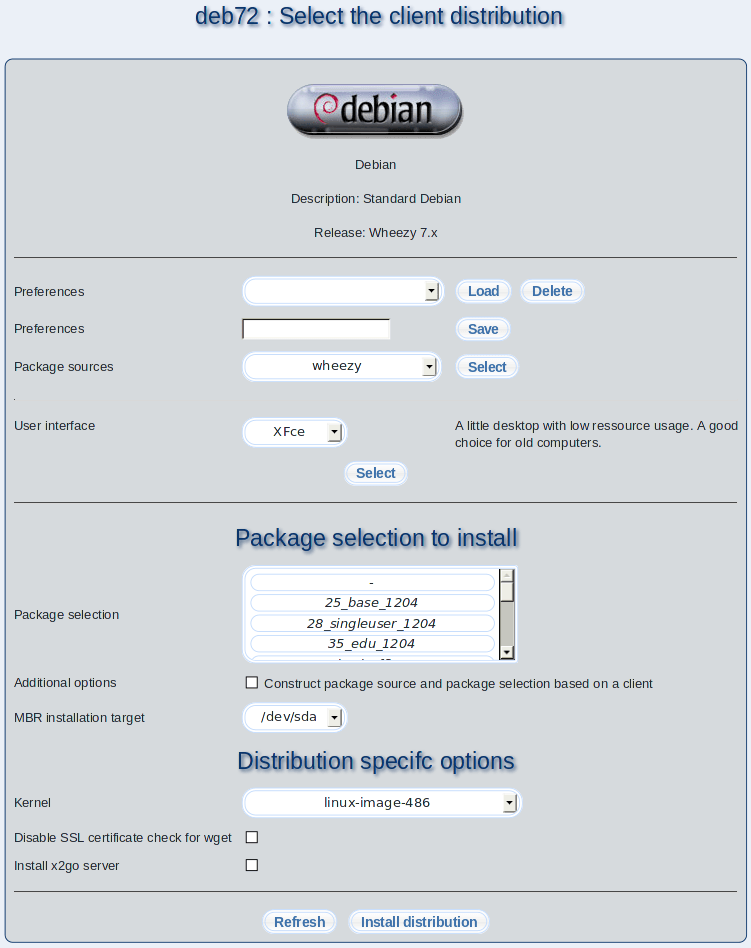
\includegraphics[scale=0.4]{/mdk/doc/manual/screenshots/de/client_distr.png} \\
Eine Distribution ist eine Zusammenstellung von verschiedenen Softwarepaketen, die auf unterschiedlichen Medien (CD, DVD, Internet) vertrieben werden. Es gibt Distributionen, die frei sind und zum kostenlosen Download im Internet angeboten werden. Ein Beispiel daf�r ist  Debian. Unterschiede bei den Distributionen bestehen lediglich in den eingesetzten Installationsprogrammen und der grafischen Aufmachung der Desktops. Die Auswahl einer Distribution ist meist reine Geschmackssache. Um die Unterst�tzung von verschiedenen Client-Distributionen in m23 zu erm�glichen, gibt es nun diesen Auswahl-Dialog.\\
\begin{itemize}
	\item \textbf{Voreinstellungen laden}: W�hlen Sie dazu eine zuvor abgespeicherte Voreinstellung aus der Auswahlliste aus und klicken Sie auf \textit{"Laden"}.\\
	\item \textbf{Voreinstellungen l�schen}: Sie k�nnen eine ausgew�hlte Voreinstellung l�schen, indem Sie auf \textit{"L�schen"} klicken.\\
	\item \textbf{Voreinstellungen speichern}: Die aktuellen Einstellungen k�nnen Sie als Voreinstellung speichern, indem Sie einen Namen eingeben und danach auf \textit{"Speichern"} klicken.\\
	\item \textbf{Paketquellenliste}: Zuerst m�ssen Sie eine Paketquelle ausw�hlen, die Sie unter \textit{Pakete} $\rightarrow$ \textit{Paketquellenliste} erstellt haben. Mit Auswahl der Paketquelle werden gleichzeitig die Distribution, das Release sowie die w�hlbaren Benutzeroberfl�chen festgelegt. Klicken Sie dazu auf \textit{"W�hlen"}. Danach wird das Logo der Distribution zusammen mit einer kurzen Beschreibung oben angezeigt.\\
	\item \textbf{Benutzeroberfl�che}: Abh�ngig von der Paketquelle k�nnen Sie verschiedene Grafische Oberfl�chen ausw�hlen. Alternativ steht \textit{"Textmode"} zur Verf�gung, um einen Server zu installieren, der keinen grafischen Desktop ben�tigt.\\
	\item \textbf{Paketzusammenstellung}: Sie k�nnen hier eine Paketzusammenstellung w�hlen, die zusammen mit dem Betriebssystem installiert wird.\\
	\item \textbf{MBR-Installationsziel}: m23 versucht automatisch die erste Festplatte f�r die Installation des Bootmanagers zu bestimmen. M�chten Sie eine hiervon abweichende Festplatte verwenden, so k�nnen Sie diese hier ausw�hlen. Bedenken Sie, da� dies die Festplatte sein mu�, die vom BIOS zum Booten verwendet wird.\\
	\item \textbf{Distributions-spezifische Einstellungen}: Jede Distribution kann eine Vielzahl von Optionen definieren, die dann zur Installation dieser Distribution genutzt werden.\\
\end{itemize}
Zum Starten der Installation klicken Sie abschlie�end auf \textit{"Distribution installieren"}.\\
\subsection{Hinweis zu Abbilddateien}
W�hlen Sie die Paketquellenliste \textit{"imaging"}, um Abbilddateien zu installieren.\\
Zus�tzlich haben Sie die Wahl, ob Sie den MBR (Master Boot Record) aus einer zuvor erstellten Datei oder den generischen MBR von m23 installieren m�chten, der bootf�hige Partitionen startet. W�hlen Sie hierzu unter \textit{"MBR aus einem Abbild oder generischen MBR installieren"} den Dateinamen oder \textit{"Generischer MBR"}.\\
\subsection{Hinweis:}
Speichern Sie eine Voreinstellung unter dem gleichen Namen ab, unter dem Sie schon Voreinstellungen f�r einen Client gespeichert haben, dann werden die Einstellungen der Distribution hinzugef�gt. Distributions-Einstellungen werden in diesem Fall �berschrieben.\\

\section{Effacer un poste client}
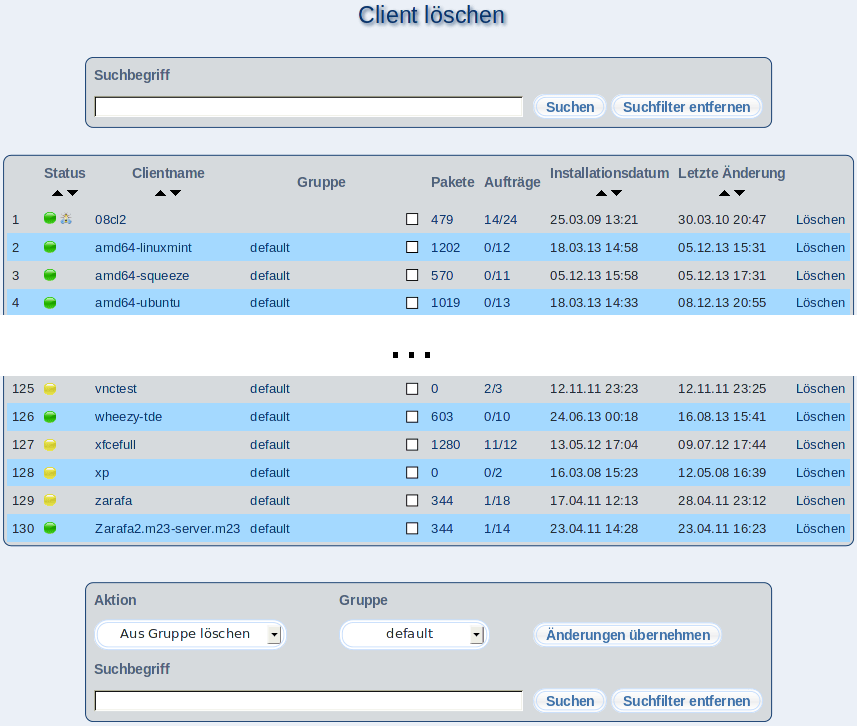
\includegraphics[scale=0.4]{/mdk/doc/manual/screenshots/fr/clients_delete.png} \\
Affin d'effacer un poste client, cliquez sur \textit{$\ll$Effacer$\gg$}. Dans le dialogue suivant, vous pouvez vous assurer qu'il s'agit du poste client correct.\\
Quand vous cliquez sur le nom d'un client, vous recevrez des informations d�taill�es sur le client s�lectionn� et vous auriez acc�s au centre de contr�le.\\
\subsection{Signification des couleurs symboliques}
Le couleur du symbol d'�tat indique l'�tat de l'installation du poste client.\\
\begin{itemize}
\item \textbf{rouge}: Le poste client a �t� ajout� et la d�tection du mat�riel automatique n'est pas encore termin�e.\\
\item \textbf{jaune}: Vous pouvez formater et partitionner le poste client, le syst�me de base sera assign� automatiquement.\\
\item \textbf{vert}: Le syst�me de base du poste client est �tabli et vous pouvez installer du logiciel suppl�mentaire.\\
\item \textbf{bleu}: Le poste client est en train d'installer du logiciel suppl�mentaire.\\
\item \textbf{orange}: Le poste client est dans un \textbf{�tat critique}. Cela veut dire qu'il y a eu une erreur pendant l'installation qui doit �tre �cart�e par l'administrateur. Au centre de contr�le, il y a des possibilit�s diff�rentes d'�carter l'�tat critique.\\
\item \textbf{blanc}: Poste client mod�le pour l'installation de masse dont les configurations seront transmis aux autres postes client.\\
\item \textbf{Mouche (bogue)}: Indique que le poste client se trouve en �tat de d�bogage.\\
\end{itemize}
\subsection{Travaux}
Dans cette colonne, vous trouvez le nombre des t�ches pas encore acomplies devant et le nombre de toutes les t�ches apr�s la barre oblique.\\
\subsection{Travailler plusieurs postes clients}
Vous pouvez choisir plusieurs postes client en mettant un crochet dans la colonne avec les postes clients souhait�s.\\
Puis, vous pouvez exercer des actions diff�rentes avec les postes client choisis:\\
\begin{itemize}
	\item \textbf{Effacer d'un groupe}: S�lectionnez le groupe duquel vous voulez effacer les postes client. Si un poste client n'appartient pas � ce groupe, aucune action sera excerc� avec lui.\\
	\item \textbf{Ajouter � un groupe}: S�lectionnez le groupe auquel vous voulez ajouter les postes client. Si un poste client appartient d�j� � ce groupe, rien ne sera chang� � sa d�pendance.\\
	\item \textbf{Effacer}: Efface les postes client s�lectionn�s\\
\end{itemize}
\subsection{Notez}
Pour voir l'�tat actuel de vos postes client, utilisez la fonction de rechargement de votre navigateur web (par exemple en appuyant sur la touche F5)\\
\subsection{Astuces}
En cliquant sur le symbole d'�tat d'un poste client, vous pouvez changer l'�tat actuel du poste client. Quand m�me, vous devriez seulement changer l'�tat d'un poste client si vous savez exactement ce que vous faites.\\
Le mode de d�bogage peut �tre (d�s)activ� par un clic sur le symbole avec la mouche.\\

\section{Client integrieren}
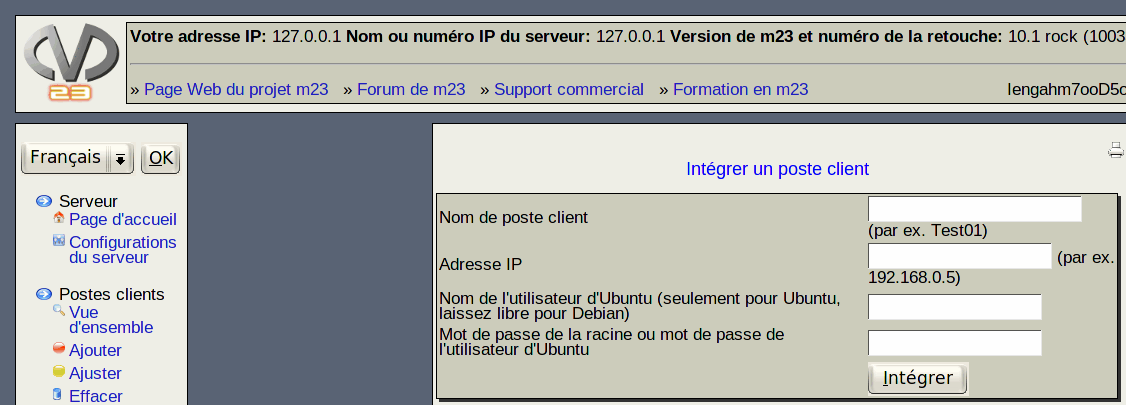
\includegraphics[scale=0.4]{/mdk/doc/manual/screenshots/de/client_assimilate.png} \\
Sie k�nnen bestehende Debian-Systeme mit m23 administrieren, indem Sie sie integrieren und somit m23 bekannt machen. F�r eine reibungslose Integration ist es erforderlich, da� der Client komplett hochgefahren und �ber das Netzwerk erreichbar ist. Nun werden nur noch drei Angaben ben�tigt:\\
\begin{itemize}
\item \textbf{Clientname}: Geben Sie hier einen Namen an, �ber den der Client im m23-Server verwaltet werden soll. Dieser Name mu� nicht zwangsl�ufig mit dem Hostnamen des Clients identisch sein.\\
\item \textbf{IP-Adresse}: Dies ist die (ggf. tempor�re) IP-Adresse des Clients.\\
\item \textbf{Name des Ubuntu-Benutzers (nur bei Ubuntu-Systemen, bei Debian leerlassen)}: Geben Sie hier einen Benutzernamen an, der auf dem Rechner ein Konto besitzt und mit dem man sich per SSH einloggen kann. Au�erdem mu� dieser Benutzer mittels sudo und seinem Pa�wort Befehle als root ausf�hren k�nnen. Dies wird nur bei Computern ben�tigt, auf denen Ubuntu installiert ist oder bei denen das Einloggen als root deaktiviert ist.\\
\item \textbf{Root-Pa�wort oder Pa�wort des Ubuntu-Benutzers}: Das aktuelle Root-Pa�wort des Clients bei Debian-Systemen oder das Pa�wort eines Benutzers bei Ubuntu-Systemen. Sie k�nnen dieses Feld allerdings auch leer lassen, wenn Sie eine manuelle Integration vorziehen.\\
\end{itemize}
Klicken Sie anschlie�end auf \textit{"Integrieren"}. Die Integration l�uft nun im Hintergrund.\\
\subsection{Hinweis}
F�r eine automatische Integration wird auf der Clientseite ein laufender SSH-D�mon, der das Einloggen als "root" erlaubt, sowie das Programm "wget" und das Paket "coreutils" vorrausgesetzt. Weiterhin ist es erforderlich, da� Pakete aus dem Internet per APT installiert werden k�nnen.\\
\subsection{Manuelle Integration}
Sollte auf dem Client kein SSH-D�mon laufen, so ist es auch m�glich, den Integrationsproze� auf dem Client per Hand anzusto�en. F�hren Sie dazu folgende Befehle als "root" in der Konsole des Clients aus (serverIP dabei durch die IP des m23-Servers ersetzen):\\
\begin{verbatim}
cd /tmp; wget http://$\langle$serverIP$\rangle$/work.php -O work.php; sh work.php
\end{verbatim}
\subsection{Hinweis f�r die Integration von Ubuntu-Systemen}
Ubuntusysteme lassen sich normalerweise nur manuell integrieren, da bei der Standardinstallation  kein laufender SSH-D�mon vorhanden ist. Starten Sie deshalb auf dem Ubuntu-Rechner eine Root-Konsole und beginnen Sie mit der manuellen Integration.\\


\chapter{Virtualisation}
\input{../createVM.hlp.tex}
\input{../downloadVBoxAddons.hlp.tex}

\chapter{Administration des groupes}
\section{Vue d'ensemble des groupes}Sur cette page, vous voyez vos groupes de postes client et le nombre de postes client y appartenants. Apr\`es un clic sur le nom d'un groupe, vous verrez la page avec les d\'etails sur le groupe respectif.\\
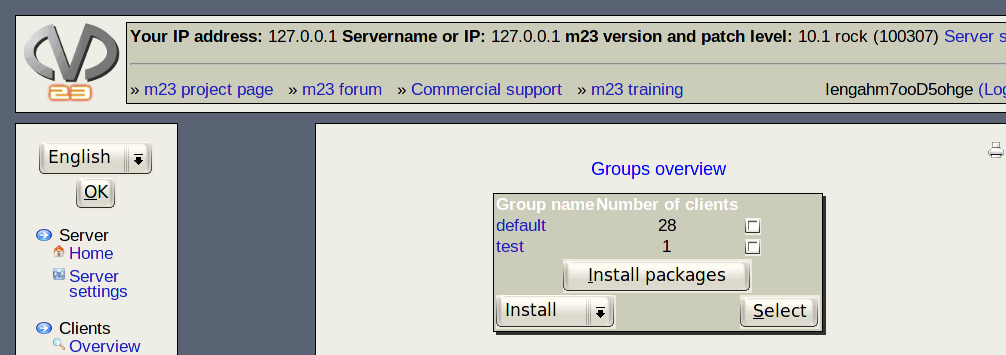
\includegraphics[scale=0.4]{/mdk/doc/manual/screenshots/fr/groups_overview.png} \\
\subsection{Donner des t\^aches \`a un groupe}
Vous pouvez donner des t\^aches aux postes client d'un ou de plusieurs groupes et, de cette fa\c{c}on, faciliter beaucoup l'administration durant l'installation, la d\'esinstallation ou la mise \`a jour.\\
\subsection{Proc\'edez comme c'est d\'ecrit au suivant:}
\begin{enumerate}
\item Choisissez l'action souhait\'ee de la liste.\\
\item Cliquez sur \textit{$\ll$Choisir$\gg$} et puis, le bouton d'action va afficher l'action choisie.\\
\item S\'electionnez le(s) groupe(s).\\
\item Enfin, double-cliquez sur le bouton d'action.\\
\end{enumerate}

\section{Ajouter un groupe}Ici, vous pouvez ajouter un groupe auquel vous pouvez assigner des postes client. En utilisant des groupes, l'administration de plusieurs postes client avec du logiciel identique est beaucoup facilit\'ee.\\
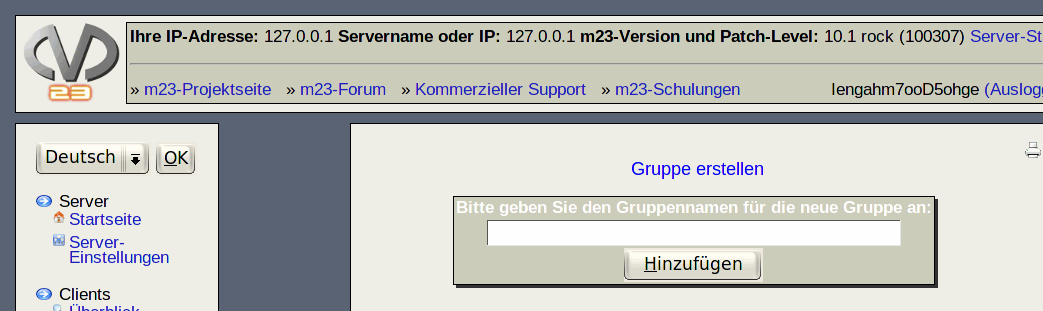
\includegraphics[scale=0.4]{/mdk/doc/manual/screenshots/fr/create_group.png} \\


\chapter{Paquets}
\section{Install packages}
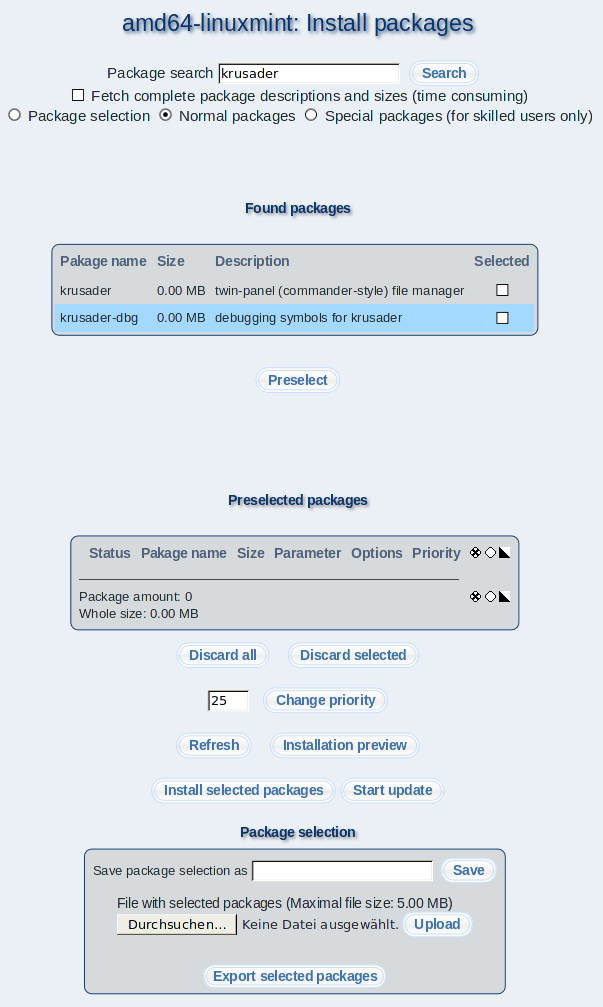
\includegraphics[scale=0.4]{/mdk/doc/manual/screenshots/en/install_packages.png} \\
\subsection{Hint}
m23 differentiates between three kinds of packages:\\
\begin{itemize}
\item \textbf{Package selection:} Are a selection of different software packages. You can make selections like \textit{"office selection"} or \textit{"graphic workstation selection"}. So you don't have to select each single software package but you can use the package selection.\\
\item \textbf{Normal packages:} Are the normal software packages. They are mostly single applications.\\
\item \textbf{Special packages (for skilled users only):} Are packages for special tasks like formatting, setting of network options etc. Special packages should only be used by skilful users.\\
\end{itemize}
\subsection{Installation of packages:}
\begin{enumerate}
\item  Select \textit{"Package selection"}, \textit{"Normal packages"} or \textit{"Special packages (for skilled users only)"}.\\
\item  Enter your search key at \textit{"Package search"}. If you leave the field blank all packages matching the package criteria are displayed. Please note that this doesn't work if you select \textit{"Normal packages"} because of the huge amount of normal packages.\\
\item  At \textit{"Found packages"} you can see all packages matching your search criteria.\\
\item  Check the checkbox beside all the packages you want to install.\\
\item  Preselect your chosen packages by clicking on \textit{"Preselect"}.\\
\item  Repeat step 1-5 if required.\\
\end{enumerate}
Complete the installation by clicking on \textit{"Install preselected packages"}.\\
Now you have preselected packages for installation. A green check mark shows that the package will be installed on the client and a red cross that the package will be removed. You can remove packages from the installation list by checking the packages and clicking on \textit{"Discard selected"} or all packages by clicking on \textit{"Discard all"}.\\
Install the packages with a clic on \textit{"Install selected packages"}.\\
\subsection{Installation preview}
Before you start the real installation, you can test what will happen during installation. You can check, which additional packages will be installed or if there will be problems. Simply click on the \textit{"Installation preview"} button. After some time you will see the previewed installation protocol.\\
An installation preview works for a single client only.\\
\subsection{Hint for package selections}
If you select a package selection, you can choose the action for the packages. You have the possibility to install or deinstall the packages on or from the client. Or you can keep the stored action. This makes it possible to store installation and deinstallation jobs in the same package selection. Simply select the desired action from the selection list.\\
\subsection{Hint}
If you want to save your package selection, enter a name for the selection at \textit{"Save package selection as"} and click the \textit{"Save"} button. Afterwards, you can use your selection as a \textit{"Package selection"}.\\

\section{Pakete deinstallieren}In diesem Dialog k�nnen Sie Pakete von einem Client entfernen.\\
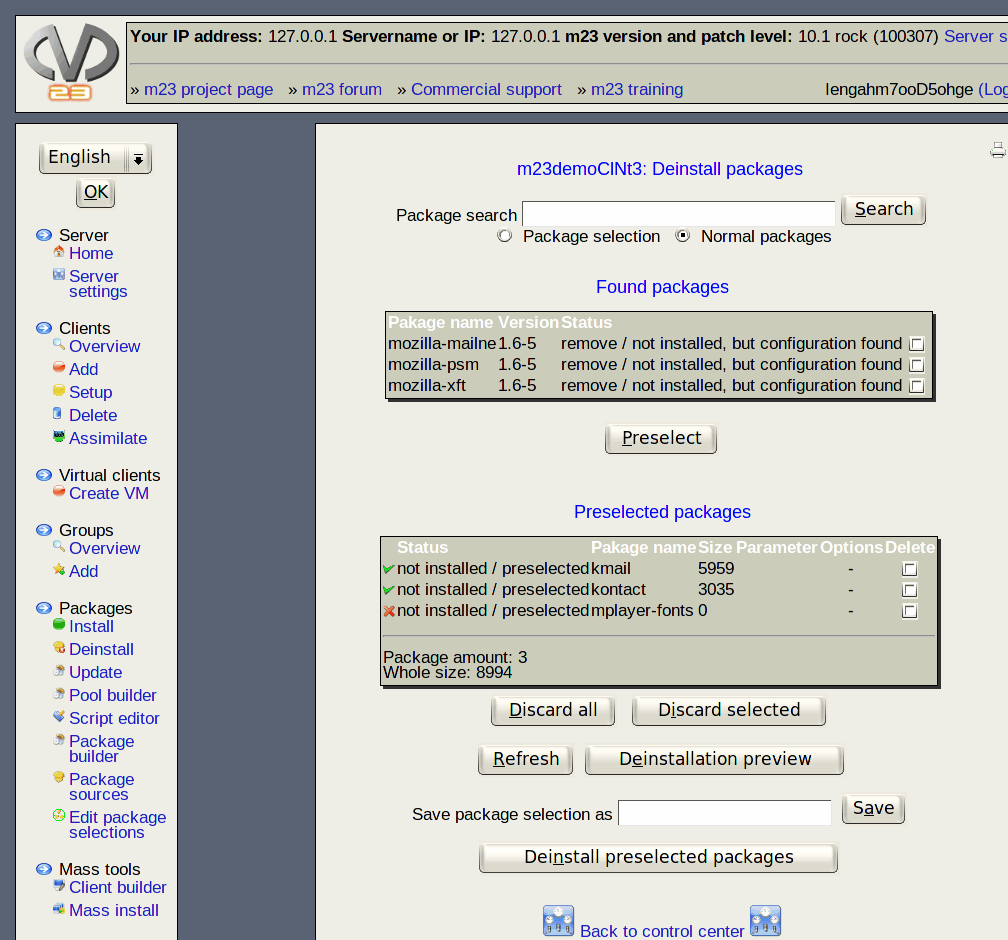
\includegraphics[scale=0.4]{/mdk/doc/manual/screenshots/de/deinstall_packages.png} \\
\subsection{Hinweis}
m23 unterscheidet drei verschiedene Paketarten:\\
\begin{itemize}
\item \textbf{Paketzusammenstellungen:} Sind eine Zusammenstellung von verschiedenen Paketen. Sie k�nnen aus einer Vielzahl von Anwendungen ein Paket schn�ren und so die Installation von identischen Programmpaketen auf verschiedenen Rechnern enorm erleichtern.\\
\item \textbf{Normale Pakete:} Sind normale Programmpakete. Dies sind in der Regel einzelne Programme.\\
\item \textbf{Spezialpakete (f�r erfahrene Benutzer):} Enthalten Pakete, die Spezialaufgaben wie Formatieren etc. durchf�hren. Spezialpakete sollten nur durch erfahrene Benutzer angewendet werden.\\
\end{itemize}
\subsection{Deinstallation von Paketen}
\begin{enumerate}
\item  W�hlen Sie \textit{"Paketzusammenstellungen"} oder \textit{"Normale Pakete"} aus.\\
\item  Geben Sie bei \textit{"Paketsuche"} den Suchbegriff f�r das gew�nschte Paket ein. Lassen Sie das Suchfeld leer, wenn Sie alle Pakete des Clients sehen m�chten.\\
\item  Unter \textit{"gefundene Pakete"} finden Sie alle Pakete, die Ihren Suchparametern entsprechen.\\
\item  Klicken Sie bei den gew�nschten Paketen die Checkbox an.\\
\item  Merken Sie die gew�hlten Pakete durch Klick auf \textit{"Vormerken"} vor.\\
\item  Wiederholen Sie bei Bedarf Schritt 1-5.\\
\end{enumerate}
Nun haben Sie Pakete f�r die Deinstallation vorgemerkt.  Ein gr�ner Haken gibt an, da� dieses Paket zu installieren ist und ein rotes Kreuz, da� dieses Paket vom Client entfernt werden soll. Sie k�nnen die Liste dieser Pakete durch einen Klick auf den Button \textit{"Alle verwerfen"} l�schen oder Pakete ausw�hlen und diese durch \textit{"Ausgew�hlte verwerfen"} entfernen.\\
Schlie�en Sie Ihre Auswahl durch Klick auf \textit{"Vorgemerkte Pakete deinstallieren"} ab.\\
\subsection{Deinstallationsvorschau}
Vor der wirklichen Deinstallation k�nnen Sie �berpr�fen, was die Deinstallation auf dem Client f�r Folgen hat. So k�nnen Sie vorher sehen, welche zus�tzlichen Pakete entfernt werden. Klicken Sie dazu nach Auswahl der Pakete auf \textit{"Deinstallationsvorschau"}. Nach einem Augenblick sehen Sie ein Protokoll der Deinstallationsvorschau.\\
Eine Deinstallationsvorschau ist allerdings nur dann m�glich, wenn ein einzelner Client und keine Gruppe ausgew�hlt wurde.\\
\subsection{Hinweis zu Paketzusammenstellungen}
Wenn Sie "Paketzusammenstellung" ausw�hlen, k�nnen Sie bestimmen, ob die Pakete auf dem Client installiert oder deinstalliert werden sollen. Au�erdem k�nnen Sie die in der Paketzusammenstellung gespeicherte Aktionen beibehalten. Dies erlaubt es, Installations- und Deinstallations-Auftr�ge in einer einzigen Zusammenstellung zu benutzen. W�hlen Sie dazu aus der Auswahlliste die gew�nschte Aktion aus.\\
\subsection{Tip}
M�chten Sie Ihre Paketauswahl f�r sp�tere Benutzung sichern, geben Sie nach \textit{"Paketauswahl als"} einen Namen f�r Ihre Zusammenstellung ein und sichern Sie diese mit dem \textit{"Speichern"}-Button. Diese Zusammenstellung steht Ihnen sofort unter \textit{"Paketzusammenstellungen"} zur Verf�gung.\\

\section{Mise \`a jour}
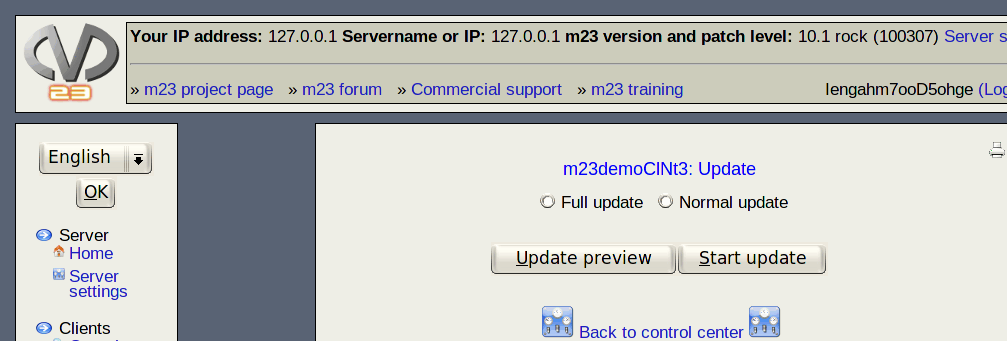
\includegraphics[scale=0.4]{/mdk/doc/manual/screenshots/fr/update_packages.png} \\
Avec la fonction de mise \`a jour, vous pouvez mettre \`a jour le logiciel sur le(s) poste(s) client. Si vous avez s\'electionn\'e un poste client singulier, vous pouvez voir une pr\'evision de la mise \`a jour.\\
\subsection{Genres de la mise \`a jour}
\begin{itemize}
\item \textbf{Mise � jour normale:} Met \`a jour les paquets install\'es et installe seulement des paquets additionels s'ils sont absolument n\'ecessaires.\\
\item \textbf{Mise � jour compl�te:} Les paquets install\'es seront mis \`a jour, des nouveaux paquets seront install\'es et des vieux paquets seront effac\'es.\\
\end{itemize}

\section{Modifier les sources de paquets}\subsection{Information}
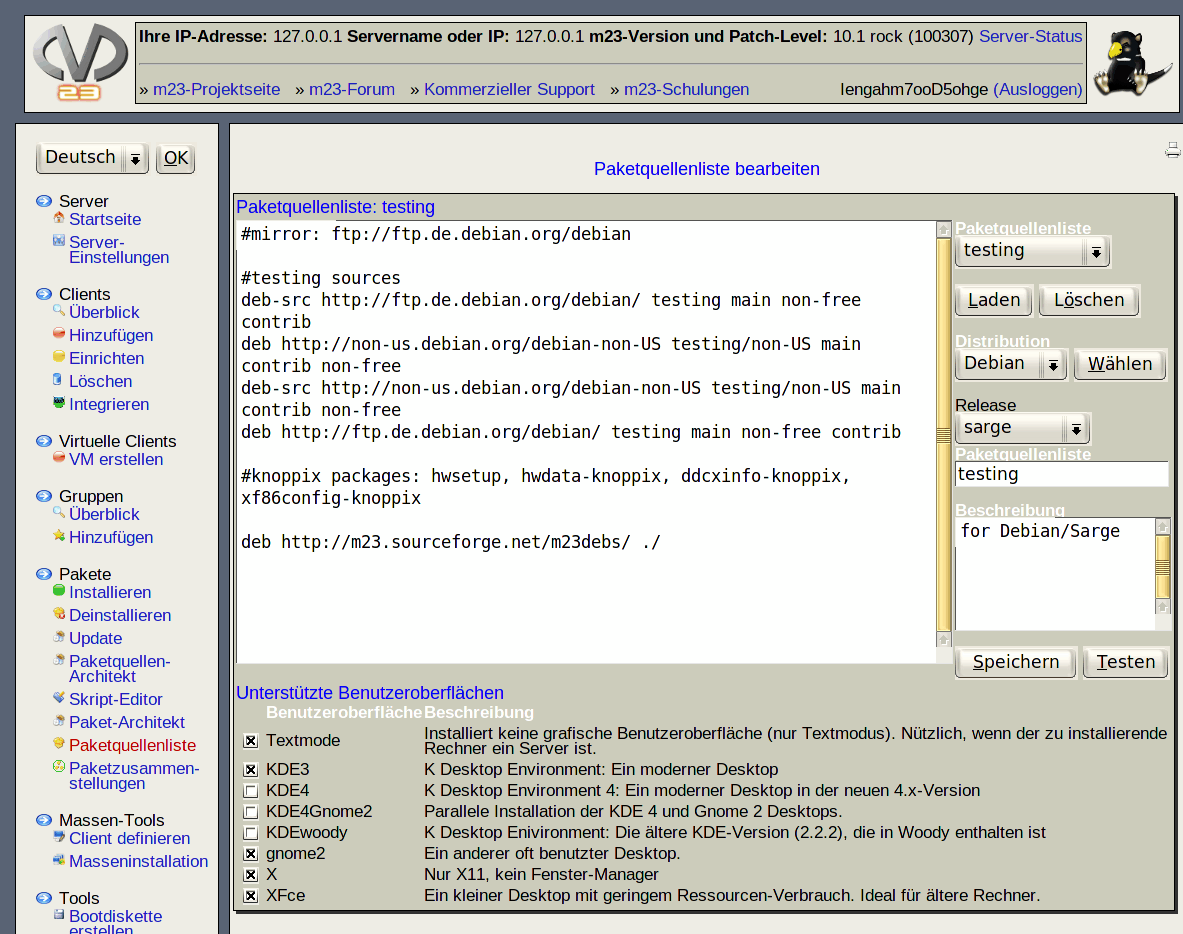
\includegraphics[scale=0.4]{/mdk/doc/manual/screenshots/fr/client_sourceslist.png} \\
Des paquets de logiciel peuvent \^etre install\'e \`a partir de diff\'erentes sources (HTTP,FTP,CDRom etc.). Des sources diff\'erentes deviennent n\'ecessaires, quand on ne peut pas installer tous les paquets de logiciel d'un medium singulier. Pour vous donner une possibilit\'e simple d'administrer les sources, vous les entrez comme vous l'\^etes habitu\'e de la distribution choisie.\\
\begin{itemize}
	\item \textbf{Charger une source de paquets}: Pour le chargement, vous choisissez la source de paquets que vous voudriez charger de la liste en haut. Apr�s un clic sur \textit{$\ll$Charger$\gg$}, elle sera charg� dans l'�diteur.\\
	\item  \textbf{Effacer une source de paquets}: Pour effacer la source de paquets charg� dans l'�diteur, cliquez sur le bouton \textit{$\ll$Effacer$\gg$} et consentiez � l'effacement au dialogue suivant.\\
	\item  \textbf{Enregistrer une source de paquets}: Il sera toujours enregistr� la source de paquets charg�e dans l'�diteur, ind�pendant de celle qui est montr�e dans la liste en haut. D'abord, choisissez la distribution � laquelle la liste des paquets doit s'appliquer. Apr�s que vous auriez choisi la distribution, il se peut passer que vous devez entrer des valeurs suppl�mentaires. En plus, s�lectionnez les interfaces graphiques support�s de la liste des sources de paquets de la liste sous la case de l'�diteur.  Trouvez un nom pour la liste de paquets et entrez-le dans le champ de saisie sous \textit{$\ll$Nom de source de paquets$\gg$}. Si vous avez charg� une source de paquets, le nom sera entr�e automatiquement. Si vous voulez, vous pouvez entrer un commentaire dans le champ \textit{$\ll$Description$\gg$}. Puis, cliquez sur \textit{$\ll$Enregistrer$\gg$}.\\
	\item  \textbf{Tester une source de paquets}: Apr�s avoir entr�e une source de paquets, vous devriez essayer si elle fonctionne conform�ment � l'ordre. Apr�s un clic sur le bouton \textit{$\ll$Tester$\gg$}, le programme essaie de t�l�charger les d�scriptions des paquets des sources. Apr�s l'ach�vement de l'essai un rapport du teste sera montr�. Il peut prendre quelques minutes jusqu'� ce que le rapport du teste apparaisse. La vitesse d�pend de votre connection � l'internet et de la vitesse des serveurs de sources de paquets utilis�s.\\
        \item \textbf{Entrer le site miroir}: Si vous voudriez utiliser un site miroir diff�rent (le site miroir de standard est ftp.debian.org) pour l'installation du syst�me de base, entrez-le dans une nouvelle ligne dans la source de paquets comme c'est d�crit au suivant: \\
\begin{verbatim}
#mirror: [URL des paquets]
\end{verbatim}
. \textit{URL des paquets} signifie le protocole, le nom d'h�te ou l'adresse IP et le r�pertoire, o� les paquets peuvent �tre trouv�s. Une ligne valide pourrait se pr�senter comme au suivant, par exemple: \\
\begin{verbatim}
#mirror: http://192.168.7.14/debianCDs
\end{verbatim}
\end{itemize}
\subsection{Information suppl\'ementaire}
\begin{itemize}
\item Si vous enregistrez une source de paquets sous un nom existant, la vieille source de paquets sera remplac\'ee.\\
\item Les \textbf{interfaces graphiques} d\'ependent directement d'une liste de sources de paquets. �a veut dire que vous pouvez uniquement utiliser les interfaces graphiques que vous avez choisis dans ce dialogue pour la liste des sources de paquets que vous voudriez utiliser pour un certain poste client. Pour cette raison, vous devriez seulement choisir les interfaces graphiques ici qui sont vraiment support\'es des sources de paquets.\\
\end{itemize}

\input{../editPackageSelection.hlp.tex}
\input{../packageBuilder.hlp.tex}
\input{../scriptEditor.hlp.tex}

\chapter{Pool builder}
\input{../poolBuilderCreateEditDelete.hlp.tex}
\input{../poolBuilderReadCD.hlp.tex}
\input{../poolBuilderCreateIndex.hlp.tex}
\input{../poolBuilderSelectPackageSourcesAndPackages.hlp.tex}
\input{../poolBuilderStartDownload.hlp.tex}
\input{../poolBuilderDownloadStatus.hlp.tex}
\input{../poolBuilderShowSourcesList.hlp.tex}

\chapter{Outils de masse}
\input{../clientBuilder.hlp.tex}
\input{../diskDefine.hlp.tex}
\section{Select value generation method}
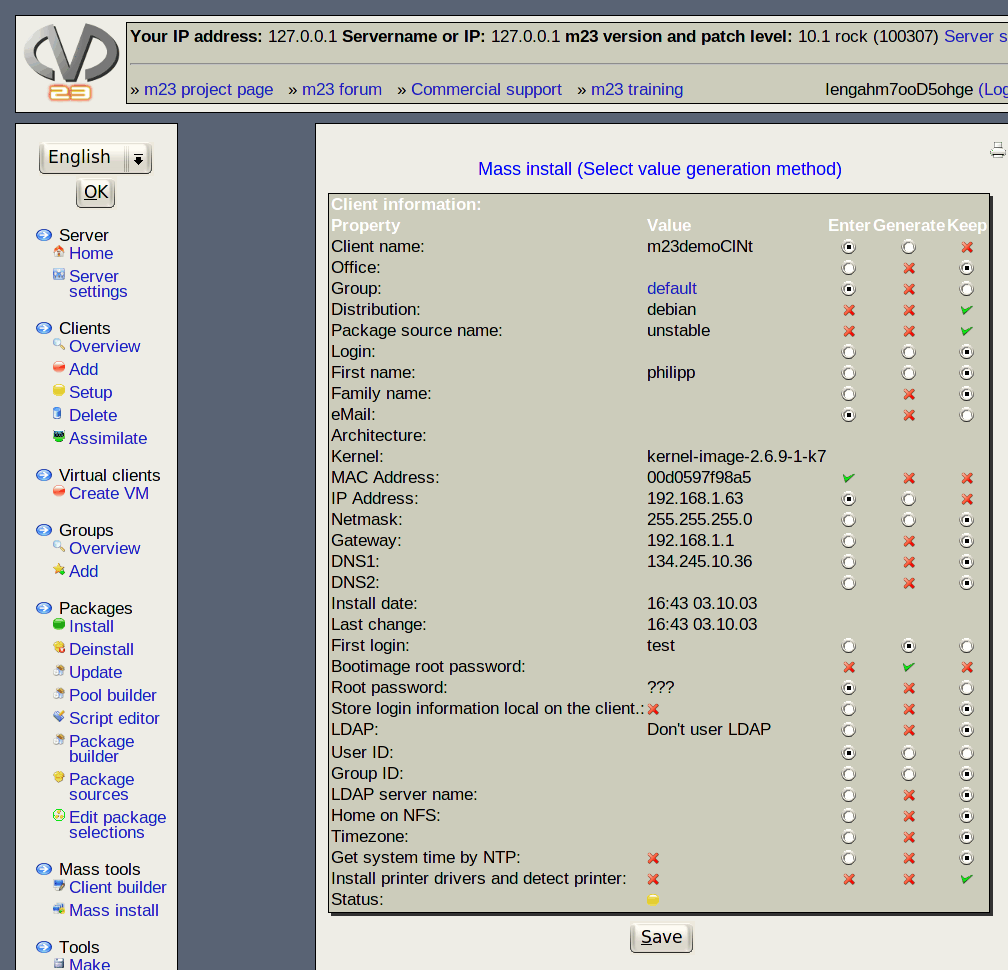
\includegraphics[scale=0.4]{/mdk/doc/manual/screenshots/en/mi_step0.png} \\
Here you can select the method for generation of the needed values.\\
\subsection{There are 3 methods}
\begin{itemize}
\item \textbf{Enter}: The values are entered by hand or read from a file.\\
\item \textbf{Generate}: The values are generated automatically. E.g. it is possible to generate client names with incrementing numbers or IP adressess with unused IP numbers.\\
\item \textbf{Keep}: The value from the "master client" is kept on all clients.\\
\end{itemize}
You don't have the possiblillity to select all 3 methods on every client option. Not selectable options are marked with a red cross. A green check shows that this method is the only one that works for this client option. E.g. it is not possible to generate MAC addresses nor to keep a MAC for all clients. MAC adresses always have to be entered by hand or read from a file.\\

\section{Choisir la source de donn\'ees}
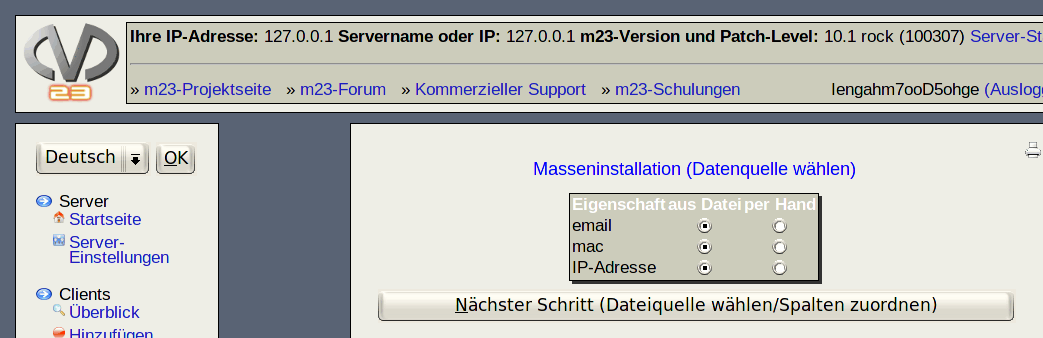
\includegraphics[scale=0.4]{/mdk/doc/manual/screenshots/fr/mi_step1.png} \\
Choisissez la source pour les propri\'et\'es qui doivent \^etre entr\'ees. Les valeurs peuvent \^etre entr\'ees en forme d'un fichier de texte ou \`a la main.\\

\section{Select data source/Assign columns}
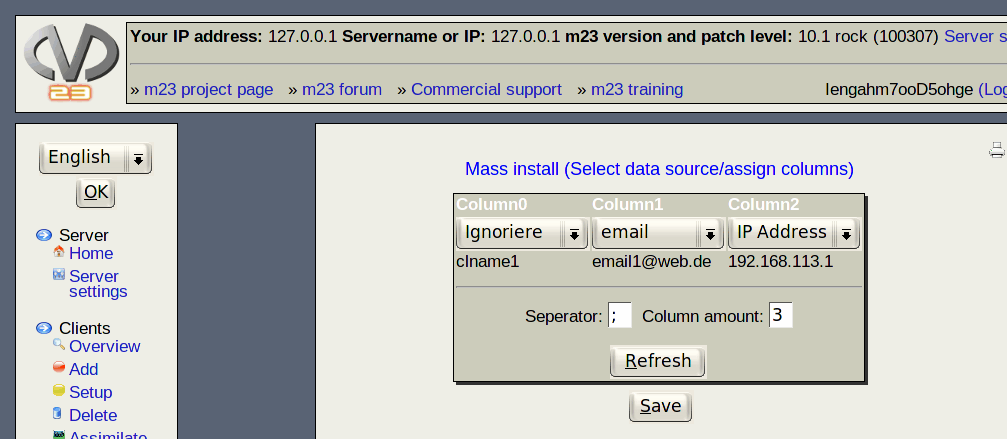
\includegraphics[scale=0.33]{/mdk/doc/manual/screenshots/en/mi_step2.png} \\
This dialog is divided into two steps:\\
\begin{itemize}
\item Select and upload a database file\\
\item Assign the fields to the client options\\
\end{itemize}
\subsection{Select and upload a database file}
Select a file with the diealog and click on \textit{"Upload"}.\\
A special data format is needed to make the value recognition possible for m23. The values for a single client are specified in every line. The client options are separated by a separator character (here ";")::\\
\begin{verbatim}
option1;option2;option3;...
\end{verbatim}
You can use other combinations of a maximum of 4 characters. The order of the options has to be the same in all lines.\\
\subsection{Hint}
All in the file stored values have to be valid and there are an additional requirements for special options:\\
\begin{itemize}
\item \textbf{Store login information local on the client.}: Set it to "yes" if you want to activate this option. All other values disable it.\\
\item \textbf{LDAP}: Here three different values are possible:\\
\begin{itemize}
\item "none": Don't user LDAP\\
\item "read": Read login information from selected LDAP server.\\
\item "write": Store login information on the selected LDAP server.\\
\end{itemize}
\end{itemize}
\subsection{Assign the fields to the client options}
You can assign the fields to the option names after uploading a file.\\
\subsection{Step by step}
\begin{enumerate}
\item Enter the separator character in the separator field and adjust the column amount if needed.\\
\item Click on \textit{"Refresh"}. The first line of the database file is now separated and shown in the client option fields.\\
\item Assign the separated parts from the database file to the client options by selecting the client option names from the selection list.\\
\item End the dialog with a click on \textit{"Save"}.\\
\end{enumerate}

\section{Generator options}
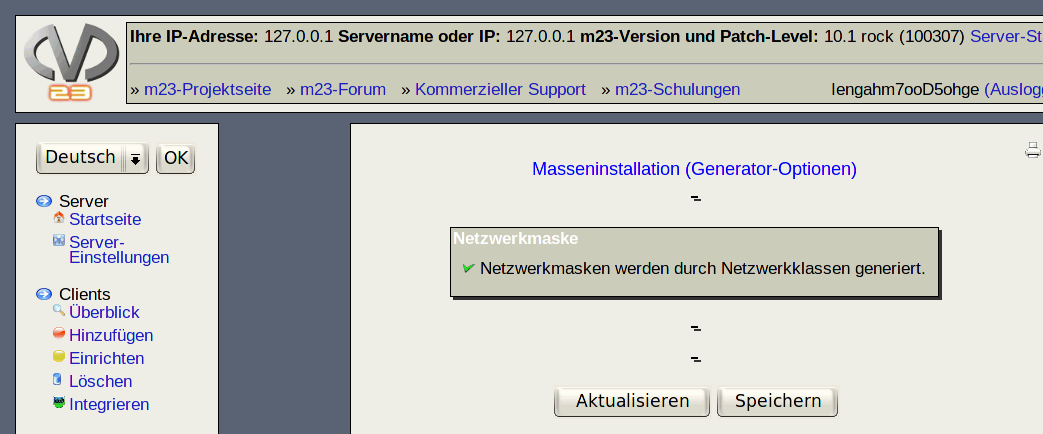
\includegraphics[scale=0.4]{/mdk/doc/manual/screenshots/en/mi_step3.png} \\
Here you can enter the values for the generators:\\
\begin{itemize}
\item \textbf{Client name}: Enter the client base name and a start number. The necessary number of client names is generated after the scheme $\langle$client base name$\rangle$$\langle$consecutive number$\rangle$. Client names already used by m23 are skipped. E.g. client base name=m23client, start number=12 generates the client names m23client12, m23client13, ...\\
\item \textbf{Login}: This is the name that is used by the user to login into the client. There are two possibilities to create login names. The incremental variant works as the method at \textit{"Client name"}. It is possible too to generate logins from the first character of the forename and the whole familyname (\textit{"Generate from fore- and familyname"}).\\
\item \textbf{First name}: The generation of the forenames (which are the login names, too) is analogical.\\
\item \textbf{IP Address}: Specify the ranges for IP addresses that should be searched for free IPs. You can activate an extra option to ping IP addresses and an IP is only used if there is no answer to the ping request. The generated IPs can be constricted by the choice of the ranges.\\
\item \textbf{Netmask}: The netmasks are generated by the defined network classes:\\
\begin{tabular}{|c|c|c|}
\hline
From & To & Netmask\\
	 \hline
0.0.0.0 & 127.255.255.255 & 255.0.0.0\\
	 \hline
128.000.000.000 & 191.255.255.255 & 255.255.0.0\\
	 \hline
192.000.000.000 & 255.255.255.255 & 255.255.255.0\\
	 \hline
\end{tabular}
\item \textbf{First login}: These passwords can be generated at random (\textit{"Random passwords"}) or random and easily memorisable for humans (\textit{"PwGen passwords"}). The length of the generated passwords can be changed. It is recommended to keep the length of 8 characters.\\
\item \textbf{User ID}: Enter the start number for the user IDs. Free IDs after this number will be used.\\
\item \textbf{Group ID}: Enter the start number for the group IDs. Free IDs after this number will be used.\\
\end{itemize}

\section{Entrer les valeurs restantes/Vue d'ensemble}Ici, vous voyez une vue d'ensemble de tous les postes client \`a cr\'eer. Maintenant, vous pouvez remplir les blancs dans les tables ou les changer et voir si les valeurs correspondent \`a vos id\'ees.\\
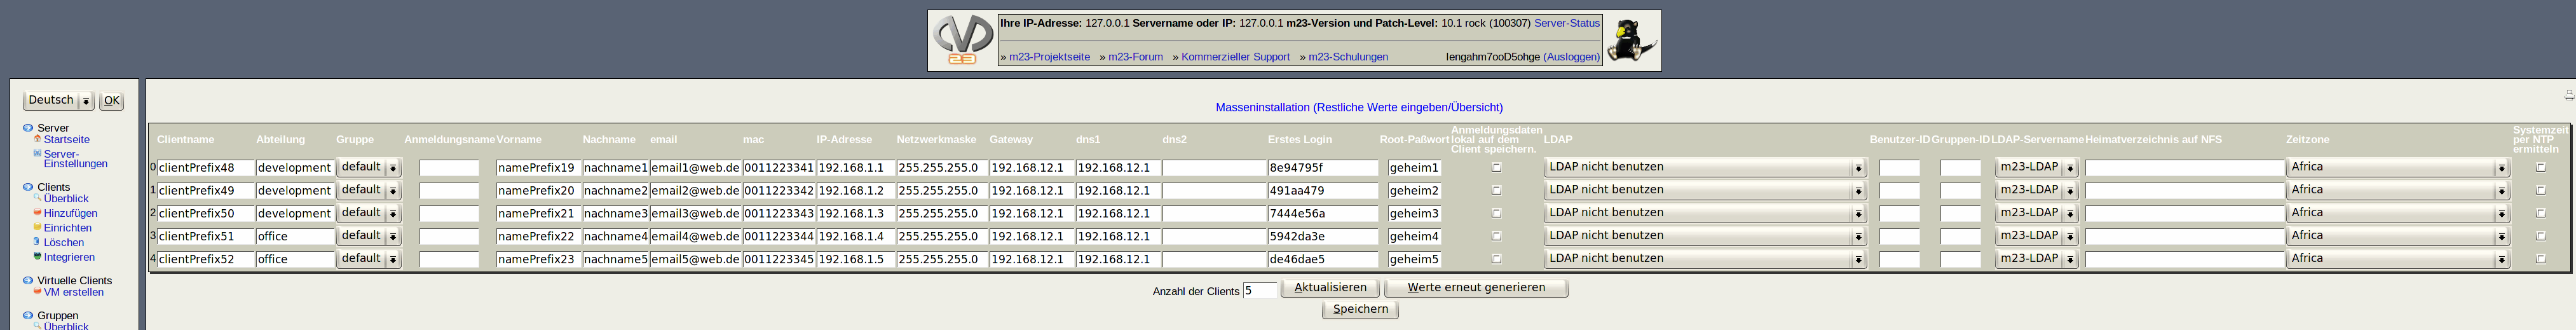
\includegraphics[scale=0.33]{/mdk/doc/manual/screenshots/fr/mi_step4.png} \\
\subsection{Changer le nombre de postes client}
Vous pouvez changer le nombre de postes client en entrant le nouveau nombre chez $\ll$Nombre de postes clients$\gg$ et puis, cliquant sur $\ll$Actualiser$\gg$, si vous d\'esirez avoir moins de postes client ou sur $\ll$G�n�rer les valeurs de nouveau$\gg$, si vous d\'esirez avoir plus de postes client.\\
Si vous d\'esirez un plus grand nombre de postes client qu'auparavant, les g\'en\'erateurs vont g\'en\'erer les valeurs n\'ecessaires apr\`es un clic sur $\ll$G�n�rer les valeurs de nouveau$\gg$ et essayer de lire les autres valeurs du fichier de banque de donn\'ees. Si le fichier de la banque de donn\'ees ne contient pas assez de valeurs, vous devez les entrer manuellement dans la table. La g\'en\'eration d'un grand nombre de valeurs peut peut-\^etre durer un long temps, par exemple si les adresses IP sont en train d'\^etre g\'en\'er\'ees et vous avez choisi que les adresses IP doivent \^etre contact\'ees avant l'usage.\\
Enfin, cliquez sur $\ll$Enregistrer$\gg$ pour commencer avec l'installation sur les postes client.\\


\chapter{Outils}
\input{../makeBootDisk.hlp.tex}
\input{../makeBootCD.hlp.tex}

\chapter{The GNU General Public License}

\begin{center}
{\parindent 0in

Version 2, June 1991

Copyright \copyright\ 1989, 1991 Free Software Foundation, Inc.

\bigskip

59 Temple Place - Suite 330, Boston, MA  02111-1307, USA

\bigskip

Everyone is permitted to copy and distribute verbatim copies
of this license document, but changing it is not allowed.
}
\end{center}

\begin{center}
{\bf\large Preamble}
\end{center}


The licenses for most software are designed to take away your freedom to
share and change it.  By contrast, the GNU General Public License is
intended to guarantee your freedom to share and change free software---to
make sure the software is free for all its users.  This General Public
License applies to most of the Free Software Foundation's software and to
any other program whose authors commit to using it.  (Some other Free
Software Foundation software is covered by the GNU Library General Public
License instead.)  You can apply it to your programs, too.

When we speak of free software, we are referring to freedom, not price.
Our General Public Licenses are designed to make sure that you have the
freedom to distribute copies of free software (and charge for this service
if you wish), that you receive source code or can get it if you want it,
that you can change the software or use pieces of it in new free programs;
and that you know you can do these things.

To protect your rights, we need to make restrictions that forbid anyone to
deny you these rights or to ask you to surrender the rights.  These
restrictions translate to certain responsibilities for you if you
distribute copies of the software, or if you modify it.

For example, if you distribute copies of such a program, whether gratis or
for a fee, you must give the recipients all the rights that you have.  You
must make sure that they, too, receive or can get the source code.  And
you must show them these terms so they know their rights.

We protect your rights with two steps: (1) copyright the software, and (2)
offer you this license which gives you legal permission to copy,
distribute and/or modify the software.

Also, for each author's protection and ours, we want to make certain that
everyone understands that there is no warranty for this free software.  If
the software is modified by someone else and passed on, we want its
recipients to know that what they have is not the original, so that any
problems introduced by others will not reflect on the original authors'
reputations.

Finally, any free program is threatened constantly by software patents.
We wish to avoid the danger that redistributors of a free program will
individually obtain patent licenses, in effect making the program
proprietary.  To prevent this, we have made it clear that any patent must
be licensed for everyone's free use or not licensed at all.

The precise terms and conditions for copying, distribution and
modification follow.

\begin{center}
{\Large \sc Terms and Conditions For Copying, Distribution and
  Modification}
\end{center}


%\renewcommand{\theenumi}{\alpha{enumi}}
\begin{enumerate}

\addtocounter{enumi}{-1}

\item 

This License applies to any program or other work which contains a notice
placed by the copyright holder saying it may be distributed under the
terms of this General Public License.  The ``Program'', below, refers to
any such program or work, and a ``work based on the Program'' means either
the Program or any derivative work under copyright law: that is to say, a
work containing the Program or a portion of it, either verbatim or with
modifications and/or translated into another language.  (Hereinafter,
translation is included without limitation in the term ``modification''.)
Each licensee is addressed as ``you''.

Activities other than copying, distribution and modification are not
covered by this License; they are outside its scope.  The act of
running the Program is not restricted, and the output from the Program
is covered only if its contents constitute a work based on the
Program (independent of having been made by running the Program).
Whether that is true depends on what the Program does.

\item You may copy and distribute verbatim copies of the Program's source
  code as you receive it, in any medium, provided that you conspicuously
  and appropriately publish on each copy an appropriate copyright notice
  and disclaimer of warranty; keep intact all the notices that refer to
  this License and to the absence of any warranty; and give any other
  recipients of the Program a copy of this License along with the Program.

You may charge a fee for the physical act of transferring a copy, and you
may at your option offer warranty protection in exchange for a fee.

\item

You may modify your copy or copies of the Program or any portion
of it, thus forming a work based on the Program, and copy and
distribute such modifications or work under the terms of Section 1
above, provided that you also meet all of these conditions:

\begin{enumerate}

\item 

You must cause the modified files to carry prominent notices stating that
you changed the files and the date of any change.

\item

You must cause any work that you distribute or publish, that in
whole or in part contains or is derived from the Program or any
part thereof, to be licensed as a whole at no charge to all third
parties under the terms of this License.

\item
If the modified program normally reads commands interactively
when run, you must cause it, when started running for such
interactive use in the most ordinary way, to print or display an
announcement including an appropriate copyright notice and a
notice that there is no warranty (or else, saying that you provide
a warranty) and that users may redistribute the program under
these conditions, and telling the user how to view a copy of this
License.  (Exception: if the Program itself is interactive but
does not normally print such an announcement, your work based on
the Program is not required to print an announcement.)

\end{enumerate}


These requirements apply to the modified work as a whole.  If
identifiable sections of that work are not derived from the Program,
and can be reasonably considered independent and separate works in
themselves, then this License, and its terms, do not apply to those
sections when you distribute them as separate works.  But when you
distribute the same sections as part of a whole which is a work based
on the Program, the distribution of the whole must be on the terms of
this License, whose permissions for other licensees extend to the
entire whole, and thus to each and every part regardless of who wrote it.

Thus, it is not the intent of this section to claim rights or contest
your rights to work written entirely by you; rather, the intent is to
exercise the right to control the distribution of derivative or
collective works based on the Program.

In addition, mere aggregation of another work not based on the Program
with the Program (or with a work based on the Program) on a volume of
a storage or distribution medium does not bring the other work under
the scope of this License.

\item
You may copy and distribute the Program (or a work based on it,
under Section 2) in object code or executable form under the terms of
Sections 1 and 2 above provided that you also do one of the following:

\begin{enumerate}

\item

Accompany it with the complete corresponding machine-readable
source code, which must be distributed under the terms of Sections
1 and 2 above on a medium customarily used for software interchange; or,

\item

Accompany it with a written offer, valid for at least three
years, to give any third party, for a charge no more than your
cost of physically performing source distribution, a complete
machine-readable copy of the corresponding source code, to be
distributed under the terms of Sections 1 and 2 above on a medium
customarily used for software interchange; or,

\item

Accompany it with the information you received as to the offer
to distribute corresponding source code.  (This alternative is
allowed only for noncommercial distribution and only if you
received the program in object code or executable form with such
an offer, in accord with Subsection b above.)

\end{enumerate}


The source code for a work means the preferred form of the work for
making modifications to it.  For an executable work, complete source
code means all the source code for all modules it contains, plus any
associated interface definition files, plus the scripts used to
control compilation and installation of the executable.  However, as a
special exception, the source code distributed need not include
anything that is normally distributed (in either source or binary
form) with the major components (compiler, kernel, and so on) of the
operating system on which the executable runs, unless that component
itself accompanies the executable.

If distribution of executable or object code is made by offering
access to copy from a designated place, then offering equivalent
access to copy the source code from the same place counts as
distribution of the source code, even though third parties are not
compelled to copy the source along with the object code.

\item
You may not copy, modify, sublicense, or distribute the Program
except as expressly provided under this License.  Any attempt
otherwise to copy, modify, sublicense or distribute the Program is
void, and will automatically terminate your rights under this License.
However, parties who have received copies, or rights, from you under
this License will not have their licenses terminated so long as such
parties remain in full compliance.

\item
You are not required to accept this License, since you have not
signed it.  However, nothing else grants you permission to modify or
distribute the Program or its derivative works.  These actions are
prohibited by law if you do not accept this License.  Therefore, by
modifying or distributing the Program (or any work based on the
Program), you indicate your acceptance of this License to do so, and
all its terms and conditions for copying, distributing or modifying
the Program or works based on it.

\item
Each time you redistribute the Program (or any work based on the
Program), the recipient automatically receives a license from the
original licensor to copy, distribute or modify the Program subject to
these terms and conditions.  You may not impose any further
restrictions on the recipients' exercise of the rights granted herein.
You are not responsible for enforcing compliance by third parties to
this License.

\item
If, as a consequence of a court judgment or allegation of patent
infringement or for any other reason (not limited to patent issues),
conditions are imposed on you (whether by court order, agreement or
otherwise) that contradict the conditions of this License, they do not
excuse you from the conditions of this License.  If you cannot
distribute so as to satisfy simultaneously your obligations under this
License and any other pertinent obligations, then as a consequence you
may not distribute the Program at all.  For example, if a patent
license would not permit royalty-free redistribution of the Program by
all those who receive copies directly or indirectly through you, then
the only way you could satisfy both it and this License would be to
refrain entirely from distribution of the Program.

If any portion of this section is held invalid or unenforceable under
any particular circumstance, the balance of the section is intended to
apply and the section as a whole is intended to apply in other
circumstances.

It is not the purpose of this section to induce you to infringe any
patents or other property right claims or to contest validity of any
such claims; this section has the sole purpose of protecting the
integrity of the free software distribution system, which is
implemented by public license practices.  Many people have made
generous contributions to the wide range of software distributed
through that system in reliance on consistent application of that
system; it is up to the author/donor to decide if he or she is willing
to distribute software through any other system and a licensee cannot
impose that choice.

This section is intended to make thoroughly clear what is believed to
be a consequence of the rest of this License.

\item
If the distribution and/or use of the Program is restricted in
certain countries either by patents or by copyrighted interfaces, the
original copyright holder who places the Program under this License
may add an explicit geographical distribution limitation excluding
those countries, so that distribution is permitted only in or among
countries not thus excluded.  In such case, this License incorporates
the limitation as if written in the body of this License.

\item
The Free Software Foundation may publish revised and/or new versions
of the General Public License from time to time.  Such new versions will
be similar in spirit to the present version, but may differ in detail to
address new problems or concerns.

Each version is given a distinguishing version number.  If the Program
specifies a version number of this License which applies to it and ``any
later version'', you have the option of following the terms and conditions
either of that version or of any later version published by the Free
Software Foundation.  If the Program does not specify a version number of
this License, you may choose any version ever published by the Free Software
Foundation.

\item
If you wish to incorporate parts of the Program into other free
programs whose distribution conditions are different, write to the author
to ask for permission.  For software which is copyrighted by the Free
Software Foundation, write to the Free Software Foundation; we sometimes
make exceptions for this.  Our decision will be guided by the two goals
of preserving the free status of all derivatives of our free software and
of promoting the sharing and reuse of software generally.

\begin{center}
{\Large\sc
No Warranty
}
\end{center}

\item
{\sc Because the program is licensed free of charge, there is no warranty
for the program, to the extent permitted by applicable law.  Except when
otherwise stated in writing the copyright holders and/or other parties
provide the program ``as is'' without warranty of any kind, either expressed
or implied, including, but not limited to, the implied warranties of
merchantability and fitness for a particular purpose.  The entire risk as
to the quality and performance of the program is with you.  Should the
program prove defective, you assume the cost of all necessary servicing,
repair or correction.}

\item
{\sc In no event unless required by applicable law or agreed to in writing
will any copyright holder, or any other party who may modify and/or
redistribute the program as permitted above, be liable to you for damages,
including any general, special, incidental or consequential damages arising
out of the use or inability to use the program (including but not limited
to loss of data or data being rendered inaccurate or losses sustained by
you or third parties or a failure of the program to operate with any other
programs), even if such holder or other party has been advised of the
possibility of such damages.}

\end{enumerate}


\begin{center}
{\Large\sc End of Terms and Conditions}
\end{center}


\pagebreak[2]

\section*{Appendix: How to Apply These Terms to Your New Programs}

If you develop a new program, and you want it to be of the greatest
possible use to the public, the best way to achieve this is to make it
free software which everyone can redistribute and change under these
terms.

  To do so, attach the following notices to the program.  It is safest to
  attach them to the start of each source file to most effectively convey
  the exclusion of warranty; and each file should have at least the
  ``copyright'' line and a pointer to where the full notice is found.

\begin{quote}
one line to give the program's name and a brief idea of what it does. \\
Copyright (C) yyyy  name of author \\

This program is free software; you can redistribute it and/or modify
it under the terms of the GNU General Public License as published by
the Free Software Foundation; either version 2 of the License, or
(at your option) any later version.

This program is distributed in the hope that it will be useful,
but WITHOUT ANY WARRANTY; without even the implied warranty of
MERCHANTABILITY or FITNESS FOR A PARTICULAR PURPOSE.  See the
GNU General Public License for more details.

You should have received a copy of the GNU General Public License
along with this program; if not, write to the Free Software
Foundation, Inc., 59 Temple Place - Suite 330, Boston, MA  02111-1307, USA.
\end{quote}

Also add information on how to contact you by electronic and paper mail.

If the program is interactive, make it output a short notice like this
when it starts in an interactive mode:

\begin{quote}
Gnomovision version 69, Copyright (C) yyyy  name of author \\
Gnomovision comes with ABSOLUTELY NO WARRANTY; for details type `show w'. \\
This is free software, and you are welcome to redistribute it
under certain conditions; type `show c' for details.
\end{quote}


The hypothetical commands {\tt show w} and {\tt show c} should show the
appropriate parts of the General Public License.  Of course, the commands
you use may be called something other than {\tt show w} and {\tt show c};
they could even be mouse-clicks or menu items---whatever suits your
program.

You should also get your employer (if you work as a programmer) or your
school, if any, to sign a ``copyright disclaimer'' for the program, if
necessary.  Here is a sample; alter the names:

\begin{quote}
Yoyodyne, Inc., hereby disclaims all copyright interest in the program \\
`Gnomovision' (which makes passes at compilers) written by James Hacker. \\

signature of Ty Coon, 1 April 1989 \\
Ty Coon, President of Vice
\end{quote}


This General Public License does not permit incorporating your program
into proprietary programs.  If your program is a subroutine library, you
may consider it more useful to permit linking proprietary applications
with the library.  If this is what you want to do, use the GNU Library
General Public License instead of this License.


\end{document}

